\documentclass{article}

% if you need to pass options to natbib, use, e.g.: \PassOptionsToPackage{numbers, compress}{natbib}
% before loading nips_2016
% to avoid loading the natbib package, add option nonatbib: \usepackage[nonatbib]{nips_2016}

\PassOptionsToPackage{numbers, compress}{natbib}
\usepackage{nips_2016}
% to compile a camera-ready version, add the [final] option, e.g.:
%\usepackage[final]{nips_2016}

\usepackage[utf8]{inputenc} % allow utf-8 input
\usepackage[T1]{fontenc}    % use 8-bit T1 fonts
\usepackage{hyperref}       % hyperlinks
\usepackage{url}            % simple URL typesetting
\usepackage{booktabs}       % professional-quality tables
\usepackage{amsfonts}       % blackboard math symbols
\usepackage{nicefrac}       % compact symbols for 1/2, etc.
\usepackage{microtype}      % microtypography
\usepackage{graphicx}
\usepackage{caption}
\usepackage{subcaption}

\usepackage{amsmath,amsthm,color,graphicx,verbatim,listings,enumitem}
\usepackage[]{algorithm2e}
\graphicspath{{figures/}}

\lstset{
numbers=left, 
numberstyle=\small, 
numbersep=8pt, 
frame = single, 
language=matlab, 
framexleftmargin=20pt}

\newtheorem{lemma}{Lemma}
\newtheorem{theorem}{Theorem}

\title{A Simple Minibatch Acceptance Test for MCMC}

% The \author macro works with any number of authors. There are two commands used to separate the
% names and addresses of multiple authors: \And and \AND.
% Using \And between authors leaves it to LaTeX to determine where to break the lines. Using \AND
% forces a line break at that point. So, if LaTeX puts 3 of 4 authors names on the first line, and
% the last on the second line, try using \AND instead of \And before the third author name.

%%  David S.~Hippocampus\thanks{Use footnote for providing further
%%    information about author (webpage, alternative
%%    address)---\emph{not} for acknowledging funding agencies.} \\
%%  Department of Computer Science\\
%%  Cranberry-Lemon University\\
%%  Pittsburgh, PA 15213 \\
%%  \texttt{hippo@cs.cranberry-lemon.edu} \\


\author{
  Haoyu Chen \\
  Department of Computer Science \\
  University of California, Berkeley \\
  \texttt{haoyuchen@berkeley.edu}
  \And
  Daniel Seita \\
  Department of Computer Science \\
  University of California, Berkeley \\
  \texttt{seita@berkeley.edu}
  \And
  Xinlei Pan \\
  Department of Bioengineering \\
  University of California, Berkeley \\
  \texttt{xinleipan@berkeley.edu}
  \And 
  Biye Jiang \\
  Department of Computer Science \\
  University of California, Berkeley \\
  \texttt{bjiang@berkeley.edu}
  \And
  John Canny \\
  Department of Computer Science \\
  University of California, Berkeley \\
  \texttt{canny@berkeley.edu}
}

\begin{document}
\maketitle

\begin{abstract}
Markov chain Monte Carlo (MCMC) methods have many applications in
machine learning. We are particularly interested in their application
to modeling very large datasets where it is impractical to perform
Metropolis-Hastings tests on the full data. We describe a novel
acceptance test which can be applied to fixed-size minibatches of
data. Previous works on reducing sample count for the
Metropolis-Hastings test require a data-dependent number of samples
which is not fixed a-priori.  They do not work on bounded-size samples
and therefore do not provide the typical practical benefits of
minibatch methods.  Our novel test requires an upper bound on the
variance of the log probability, but given this condition it can be
applied to fixed-size minibatches of data. We show via experiments
that if this condition is not met, that the earlier methods consume an
large number of samples.  Our test is extremely simple and fast,
bringing the benefits of minibatch methods to MCMC inference.
Alternatively, the variance condition can be used to adjust the
temperature of the sampling distribution to a ``natural'' value to
provide regular samples at a given minibatch size. The resulting
proposal/test is only slightly more complex than a simple SGD
update. In this paper we derive the test, discuss its implementation,
and present several experiments.
\end{abstract}



\section{Introduction}\label{sec:introduction}

Markov chain Monte Carlo (MCMC) sampling is a powerful method for
computation on intractable distributions. MCMC algorithms propose
samples from a proposal distribution $q$ which is in general different
from the target distribution $p$, and decide whether to accept or
reject them based on an acceptance test. The acceptance test is
usually a Metropolis-Hastings
test~\cite{Metropolis1953,hastings70}. For example, for Bayesian
posterior inference, the sampling target distribution over the
parameters $\theta$ is the posterior distribution $p(\theta \mid x_1,
\ldots, x_N) \propto p(\theta)\prod_{i=1}^np(x_i \mid \theta)$ of
based on conditionally independent data $\{x_i\}_{i=1}^n$. When $n$ is
large, it is very expensive to compute the exact posterior because the
likelihood must be evaluated on every $x_i$.

Many state-of-the-art machine learning methods, and deep learning in
particular, are based on minibatch updates (such as SGD) to a model.
Minibatch updates produce many improvements to the model for each pass
over the dataset, and have high sample efficiency. They also map very
well onto hardware such as GPUs. In contrast, MCMC methods typically
require calculations over the full dataset to produce a new sample.
Recent results
\cite{cutting_mh_2014,conf/uai/MaclaurinA14,icml2014c1_bardenet14}
attempted to bridge the gap between minibatch optimization and MCMC by
data-adaptive subsampling. These methods uses a
subset of the $N$ data points for the MH test each iteration. However
the number of points is not known a priori, and is adjusted
dynamically during every test. This undermines many of the practical
advantages of minibatch calculations: GPU kernels work best for
certain minibatch sizes, memory blocks can be reused when minibatch
size is fixed, etc.

In this paper, we develop an alternative minibatch acceptance test for MCMC
methods which uses only one fixed-size minibatch per test. Instead of
dynamically adjusting the batch size, we add a prerequisite for the test
based on the variance of the log acceptance probability. If this
variance is small enough, the test requires only a single step. This
variance changes slowly on typical problems, and we can estimate it
before performing the test. The minibatch variance
decreases as the minibatch size grows, so the variance measurement can be
used to set the minimum minibatch size.

There is another advantage when using our test for Bayesian
posterior inference. As the dataset size grows, the posterior distribution
sharpens and often concentrates to a few sharp peaks. Samples from
this distribution will come from those peaks, and will easily become
stuck in one of them (see Section~\ref{ssec:gaussians}).  The samples are not exploring
the posterior parameter space, and are unlikely to concentrate at a
strong local optimum. They therefore fail to accurately represent a
sample of the posterior because of inadequate search (i.e.,
mixing). We argue that it is much more natural to sample the
distribution at a higher temperature determined by the
minibatch size rather than the dataset size. This temperature is
determined in a natural way by the variance prerequisite for our
test. Starting at a high temperature (small minibatch size) which
mixes easily, one can reduce the temperature (increasing minibatch
size) until one reaches the desired target distribution temperature.
Although this approach also involves changing minibatch size, the
changes increase minibatch size monotonically, and only a few changes
are performed in the course of a sampling session.
Annealing can also be used for MAP and ML estimation because changing temperature preserves
posterior modes. 

To be precise, the contributions of this paper are as follows:

\begin{enumerate}[noitemsep]
\item We develop a new acceptance test which works on fixed-size data samples, given
  an auxiliary condition. 
    \item We compare performance of our new test and adaptive sampling methods.
    \item We experiment using the approach for posterior estimation.
\end{enumerate}




\section{Preliminaries and Related Work}\label{sec:related_work}

In standard MCMC methods~\cite{gilks1996markov,brooks2011handbook} for Bayesian inference with
parameter $\theta$ and conditionally independent data, the goal is to compute the distribution
$p(\theta \mid x_1, \ldots, x_N)$.  To do so, one generates a chain of (correlated) samples
$\theta_1, \ldots, \theta_T$ for large $T$ and approximates $p$ using the sample counts.  Each
iteration $t$ has a current $\theta_t$, and a \emph{proposal distribution} $q(\theta' \mid
\theta_t)$ determines a new candidate $\theta'$. With probability $P_a$, the sample is accepted, so
$\theta_{t+1} = \theta'$. Otherwise, $\theta_{t+1} = \theta_t$. This is done by drawing a uniform
random variable $u \sim {\rm Unif}[0,1]$ and accepting if $u < P_a$. Traditionally, $P_a$ is
\begin{equation}\label{eq:traditional}
P_a = \min\left\{ 1, \frac{f(\theta')q(\theta_t \mid \theta')}{f(\theta_t)q(\theta' \mid \theta_t)}
\right\} = \min\left\{ 1, \frac{p(\theta')\prod_{i=1}^N p(x_i \mid \theta')q(\theta_t \mid
\theta')}{p(\theta_t)\prod_{i=1}^N p(x_i \mid \theta_t)q(\theta' \mid
\theta_t)} \right\},
\end{equation}
where $f(\theta_t)=p(\theta_t \mid x_1,\ldots,x_N)$. The $P_a$ from Equation~\ref{eq:traditional}
satisfies detailed balance, so if one samples long enough, one will arrive at a stationary
distribution matching the posterior, though a burn-in period and/or taking every $n$th sample may be
helpful.

Unfortunately, computing $f$ requires the use of all $N$ training data
points. Moreover, it is difficult to design tests using substantially
fewer than $N$ points that also satisfy detailed balance. To reconcile
these competing objectives,~\cite{cutting_mh_2014} proposes an
adaptive minibatch MCMC algorithm which uses a sequential hypothesis
test. During each iteration, the algorithm starts with a small
minibatch of data and adds additional samples until the test either
succeeds or fails. in the worst case, all $N$ data points may be
needed in a single iteration.  A similar approach is explored in
~\cite{icml2014c1_bardenet14} but as the authors there note, the
method is ``of limited usefulness'' when the log probability variance
is high, and the method may consume all or most of the samples. The
work of~\cite{conf/uai/MaclaurinA14} presents another approach to
reducing sample size for MH testing. In their case, auxiliary
variables are introduced which allow exact sampling from the
posterior. Their method assumes a lower bound on the posterior
probability. Unfortunately, in the most challenging situations (high
variance in the log probability), this lower bound, if it exists at
all, will be much smaller than the mean probability. As a consequence,
this method will consume most of the data samples.

MCMC methods can use physics-inspired state-space
extensions. By viewing random variables as particles in a physical
system and adding virtual momentum variables, one realizes the
Hamiltonian Monte Carlo (HMC)~\cite{mcmc_hamiltonian_2010} approach.
These methods generate high-efficiency proposals with large steps and
high acceptance rates. Traditional HMC methods require a full gradient
computation for proposals, but recent extensions
HMC~\cite{sghmc_2014,stochastic_thermostats_2014} use minibatches of
data. Langevin Dynamics~\cite{langevin_2011,conf/icml/AhnBW12} is a
similar approach which does not use the momentum terms in HMC, but
typically produces smaller steps and random-walk behavior. In both
cases, these methods avoided the expense of MH acceptance tests which
are much larger than the minibatch proposals. But because of this they
are forced to limit step size so that their approximate proposals
generate the true distribution in the limit. With our fast test,
these methods can be made more efficient by using larger
step sizes without compromising accuracy.
We demonstrate this in Section~\ref{ssec:nets}.

%% Daniel: for a further discussion on the 'Firefly' paper, see this blog post:
%% https://xianblog.wordpress.com/2014/04/02/firefly-monte-carlo/
%% Note: this guy also blogged about our earlier ICLR 2015 paper. He's the third author of the SAME
%% paper, which explains why he knows this stuff.




\section{A New Metropolis-Hastings Test}\label{sec:our_algorithm}

For our new MH test, we define $\Delta$ and $\Delta'$ which are logs of transition probability
ratios:
\begin{equation}\label{eq:deltas}
\Delta = \log \left( \frac{p(\theta')  \prod_{i=1}^N p(x_i \mid \theta')  q(\theta_t \mid
\theta')}{p(\theta_t)\prod_{i=1}^N p(x_i \mid \theta_t)  q(\theta' \mid
\theta_t)} \right);\;  \Delta' = \log \left( \frac{p(\theta') (\prod_{i=1}^n p(x_i \mid
\theta'))^{\frac{N}{n}} q(\theta_t \mid \theta')}{p(\theta_t) (\prod_{i=1}^n p(x_i \mid
\theta_t))^{\frac{N}{n}} q(\theta' \mid \theta_t)} \right)
\end{equation} 
where $p$ and $q$ are target and proposal distributions respectively
as in Equation~\ref{eq:traditional}. Note that the difference
between $\Delta$ and $\Delta'$ is that they use $N$ and $n$ data terms
$x_i$, respectively, and that the latter uses an $N/n$ scaling
term. The scaling term ensures that $\Delta'$ is an unbiased estimator of $\Delta$.
 We assume $n \ll N$ (so $\Delta'$ is substantially faster to
compute) and that the $n$ data points $x_i$ represent a random
minibatch of data.

\subsection{The Full Data Test}\label{ssec:deltas_full}

To motivate the use of $\Delta$, we turn to Lemma~\ref{lem:detailed_balance}.

\begin{lemma}\label{lem:detailed_balance}
Let $\Delta$ be defined as in Equation~\ref{eq:deltas}. Any acceptance function $g$ such that
$g(\Delta) = \exp(\Delta) g(-\Delta )$ satisfies detailed balance. That is, $f(\theta_t)p(\theta'
\mid \theta_t) = f(\theta')p(\theta_t \mid \theta')$, where $p(\theta_y \mid \theta_x)$ is the
probability of jumping from $\theta_x$ to $\theta_y$ in our chain.
\end{lemma}

\begin{proof}
We begin by deriving $p(\theta' \mid \theta_t)$. This is equivalent to the probability of proposing
$\theta'$ and then accepting it, so $p(\theta' \mid \theta_t) = q(\theta' \mid \theta_t)g(\Delta).$
Similarly, $p(\theta_t \mid \theta') = q(\theta_t \mid \theta')g(-\Delta).$ Notice that the
probability of accepting a transition from $\theta'$ to $\theta_t$ is $g(-\Delta)$ because this
inverts the fraction inside the logarithm term of $\Delta$.  By assumption, we can expand $g(\Delta)
= \exp(\Delta)g(-\Delta)$ in $p(\theta' \mid \theta_t)$. Doing this, and combining the result with
the definition of $p(\theta_t \mid \theta')$, we get
\begin{equation}\label{eq:combined}
g(-\Delta) = \frac{p(\theta' \mid \theta_t)}{q(\theta' \mid \theta_t)\exp(\Delta)} = \frac{p(\theta_t \mid \theta')}{q(\theta_t \mid \theta')}.
\end{equation}
Rearranging terms and expanding $\exp(\Delta)$, we have
\begin{equation}\label{eq:rearrange}
\frac{p(\theta' \mid \theta_t) f(\theta_t) q(\theta' \mid \theta_t)}{q(\theta' \mid \theta_t) f(\theta') q(\theta_t \mid \theta')} = \frac{p(\theta_t \mid \theta')}{ q(\theta_t \mid \theta')}.
\end{equation}
Cancellations result in $f(\theta') p(\theta_t \mid \theta') = f(\theta_t) p(\theta' \mid
\theta_t)$. Thus, detailed balance is satisfied.
\end{proof}

As a sanity check, the standard Metropolis-Hastings acceptance function $g(\Delta) = \min\{1,
e^\Delta \} = \min\left\{1, \frac{f(\theta')q(\theta_t \mid \theta')}{f(\theta_t)q(\theta' \mid
\theta_t)}\right\}$ satisfies the condition $g(\Delta) = \exp(\Delta)g(-\Delta)$.

For our MH test, the key is that we use a different $g$, the logistic
function: $g(\Delta) = (1+\exp(-\Delta))^{-1}$. Straightforward
arithmetic shows that it satisfies the condition in
Lemma~\ref{lem:detailed_balance}.  The logistic function is ideal for
this task because we can easily sample from it using the following
procedure: At any iteration with a current parameter $\theta_t$ and a
candidate sample $\theta'$, we can compute $\Delta$. Let $u$ be a
uniform random variable $u \sim {\rm Unif}[0,1]$. We accept $\theta'$
if $g(\Delta) > u$, and reject otherwise. This process is equivalent
to sampling a random variable $X$ with cumulative distribution
function $F_X(x) = g(x)$, and accepting if $\Delta > X$ and rejecting
otherwise. We can define $X = g^{-1}(u)$ so that its CDF is the
logistic function, which follows because for arbitrary $X = x$, we
have
\[
F_X(x) = {\rm Pr}(X \le x) = {\rm Pr}(g^{-1}(u) \le x) = {\rm Pr}(u \le g(x)) = \int_{0}^{g(x)} 1 dx = g(x),
\]
as the density of $u$ is one. Thus, the criteria to accept the candidate $\theta'$ is equivalent to
whether $\Delta > X$. Moreover, $X$ is symmetric about zero, so the acceptance criteria can also be
expressed as $\Delta + X>0$.

\subsection{The Minibatch Version}\label{ssec:deltas_minibatch}

With large datasets, $\Delta$ is intractable to compute. An intuitive fix is to instead use the
minibatch approximation $\Delta'$. The following lemma characterizes the distribution of $\Delta'$.

\begin{lemma}\label{lem:gaussian}
If the minibatch data is chosen randomly and sufficiently large, then the distribution of $\Delta'$ is approximately Normal.
\end{lemma}

\begin{proof}
By expanding the definition of $\Delta'$ from Equation~\ref{eq:deltas}, we get
\[
\Delta' = \log p(\theta') - \log p(\theta_t) + \log q(\theta_t \mid \theta') - \log q(\theta' \mid \theta_t) +
\frac{N}{n}\sum_{i=1}^n (\log p(x_i\mid \theta') - \log p(x_i\mid \theta_t)).
\]
During a given iteration, $\theta_t$ and $\theta'$ are fixed. Therefore, the variation in $\Delta'$
comes only from the samples in the minibatch. Since each term in the sum is IID, the distribution of
$\sum_{i=1}^n (\log p(x_i\mid \theta') - \log p(x_i\mid \theta_t))$ converges to a Normal distribtuion as $n
\to \infty$ by the Central Limit Theorem.
\end{proof}

% Daniel: I decided to put the figure here, so it's closer to the text that references it.
\begin{figure}[t]
    \centering
    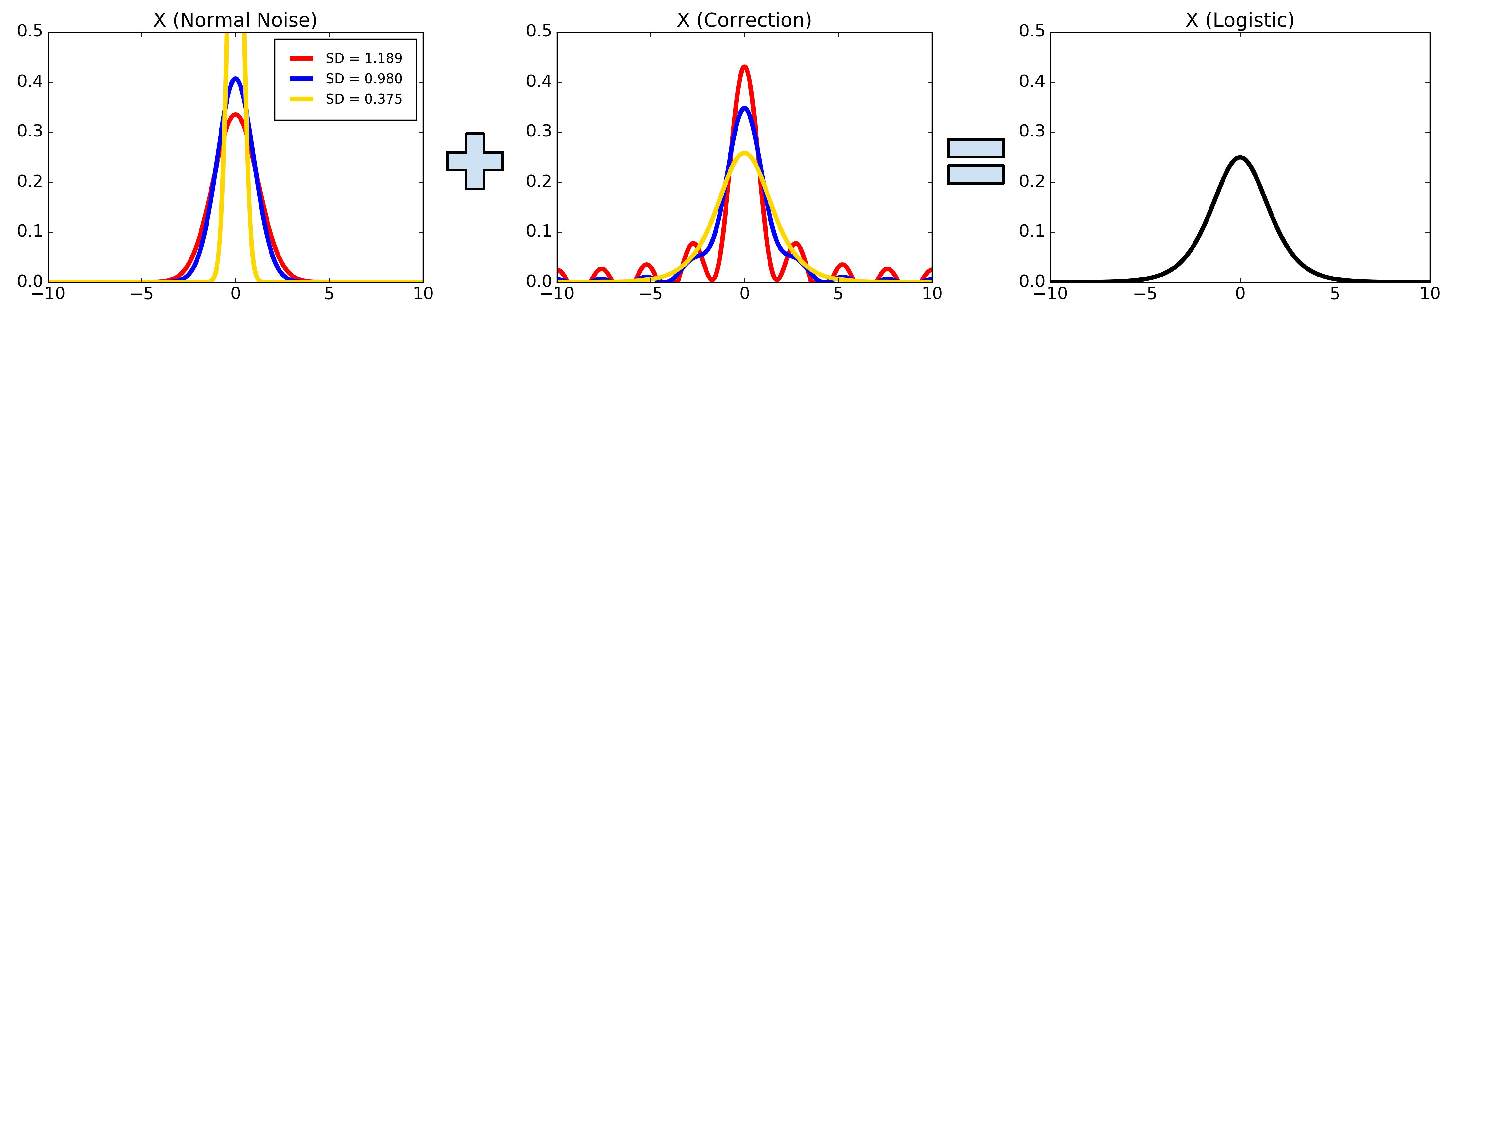
\includegraphics[width=1\textwidth]{mh_convolution_diagram_v2}
    \caption{
    Three examples of $X_{\rm norm}$ and $X_{\rm corr}$ distributions that convolve to form the
    standard logistic distribution. We use three standard deviation values of $X_{\rm norm}$. The
    two red curves convolve to form the logistic, etc. The $y$-axis is capped at 0.5 for
    readability. This figure must be viewed in color.
    }
    \label{fig:deconvolution}
    %\vspace{-10pt}
\end{figure}

From Lemma~\ref{lem:gaussian}, since $\Delta'$ is a noisy approximation of $\Delta$, the
relationship is expressed as
\begin{equation}\label{eq:relationship}
\Delta' \approx \Delta + \varepsilon, \quad \varepsilon \sim \mathcal{N}(0, \sigma^2),
\end{equation}
for a Normal noise term $\varepsilon$.  The extra noise means we can no longer directly perform
the $\Delta + X$ test, so we need to slightly change our acceptance criteria. Our insight is to
decompose $X$ as
\begin{equation}\label{eq:deconvolution}
X = X_{\rm norm}+X_{\rm corr},
\end{equation}
where we assume $X_{\rm norm}$ is a zero-mean Normally-distributed and $X_{\rm corr}$ is a zero-mean
``correction'' term.  These two add to form $X$. The criteria
to accept is now
\begin{equation}\label{eq:criteria}
\Delta + X = \Delta + X_{\rm norm} + X_{\rm corr} \approx \Delta' + X_{\rm corr} >0.
\end{equation}
The approximation exists because $X_{\rm norm}$ is an estimate of $\varepsilon$. If $X_{\rm norm}$
is exact, then we get the same MH test with $\Delta'$ as we do with the full data version $\Delta$.

Equations~\ref{eq:deconvolution} and~\ref{eq:criteria} yield an extremely simple test: Namely,
compute the approximate log transition probability ratio $\Delta'$, add the correction random
variable, and compare with zero. It remains to be determined how, and under what conditions
we can do the decomposition~\ref{eq:deconvolution}. First we recall that the distribution
of a sum of indendent random variables is the convolution of their distributions. From equation
\cite{eq:deconvolution}, we know the distributions of both $X_{\rm norm}$ and $X$. It follows
that $X_{\rm corr}$ is the {\em deconvolution} of $X$ by $X_{\rm norm}$. Such a decomposition
need not exist. For instance, \ref{eq:deconvolution} implies that
\begin{equation}
  {\rm var}(X) = {\rm var}(X_{\rm norm}) + {\rm var}(X_{\rm corr})
\end{equation}
so we must have ${\rm var}(X) > {\rm var}(X_{\rm norm})$ to have a chance of success. In fact
since these distributions are known, the variance information is enough to determine whether
the test is applicable. The correction sample can be generated as follows:

\begin{enumerate}[noitemsep]
    \item We first need to estimate the standard deviation of $X_{\rm norm}$. We generate $K$ values
    of $\Delta'$, each using a different random minibatch of $n$ data points, but each using the
    same $\theta_t$ and $\theta'$. In our experiments (see Section~\ref{sec:experiments}), $K$ is
    small, around 5-10, and $n$ is usually a few hundred for the Central Limit Theorem to apply.
    Using these $K$ values, we use the empirical standard deviation ${\rm std}(\Delta')$.

    \item Once we have ${\rm std}(\Delta')$, we can determine the distribution of $X_{\rm corr}$
    from standard deconvolution techniques. These rely on the well-known fact that the Fourier
    transform of a convolution is the product of the Fourier transforms. In practice, we pre-compute
    distributions of $X_{\rm corr}$ for different ${\rm std}(\Delta')$ values to facilitate the
    sampling process.
\end{enumerate}

Algorithm~\ref{alg:our_algorithm} describes our MH test within the MCMC algorithm.

\subsection{Discussions and Practical Considerations of the New MH Test}\label{ssec:discussion}

\SetKwInOut{Input}{Input}
\SetKwInOut{Output}{Output}
\begin{algorithm}[t]
\Input{Number of samples $T$, variance estimation window $W$, minibatch size $m$, pre-computed $X_{\rm
corr}$ distributions, $\{x_i\}_{i=1}^n$ values from a target distribution, and initial sample $\theta_0$.}
\Output{A chain of $T$ samples $\{\theta_1, \ldots, \theta_T\}$}
\For{$t=\{1, \ldots, T\}$}{
    Propose a candidate $\theta'$ and create an empty list for $\Delta'$ estimates, $d = []$\;
    \For{$k = \{1, \ldots, W\}$}{
        Sample a random minibatch of size $m$ from the complete data\;
        Compute $\Delta'$ from this minibatch (see Equation~\ref{eq:deltas}), and add $\Delta'$ to $d$\;
    }
    Compute ${\rm std}(d)$, the standard deviation estimate of $\Delta'$ from list $d$\;
    \eIf{${\rm std}(d) \ge 1.2$}{
        Skip loop (set $\theta_{t+1}=\theta_t$) and apply variance preconditioning fix (if desired)\;
    }{
        Choose the closest $X_{\rm corr}$ distribution, and sample a value $X_c$ from it\;
        Using another random minibatch of $m$ data points, compute a \emph{new} $\Delta'$ (call it $\Delta_{\rm real}'$)\;
        \eIf{$X_c + \Delta_{\rm real}' > 0$}{
            Accept the candidate, $\theta_{t+1} = \theta'$\;
        }{
            Reject and re-use the sample, $\theta_{t+1} = \theta_t$\;
        }
    }
}
\caption{A description of our MH test within the MCMC algorithm.}
\label{alg:our_algorithm}
%\vspace{-10pt}
\end{algorithm}

\textbf{The Convolution}. Figure~\ref{fig:deconvolution} demonstrates
Equation~\ref{eq:deconvolution} and provides three (color-coded) examples of densities for $X_{\rm
norm}$ and $X_{\rm corr}$. The density of $X$, a logistic random variable with mean $\mu = 0$ and
scale $s=1$, is known, as are the $X_{\rm norm}$ densities for different standard deviations. The
deconvolution provides us with the $X_{\rm corr}$ distributions. Note, however, that as the standard
deviation of $X_{\rm norm}$ increases, the $X_{\rm corr}$ distribution becomes increasingly unstable
and ``bumpier'', because the logistic curve has fatter tails than the normal distribution. For this reason, we cap
the standard deviation possibilities of $X_{\rm norm}$ at $\approx 1.2$ in our experiments. In our
experiments, we discretize the possible standard deviations of $X_{\rm norm}$, and we also limit the
densities to consider the range $[-10,10]$ (as shown in Figure~\ref{eq:deconvolution}).

\textbf{Variance Preconditioning}. Returning to the discussion from Section~\ref{sec:introduction},
our test requires a variance check. Equation~\ref{eq:deconvolution} means that the variance of $X$,
which is $\pi^2/3\approx 3.29$ is an upper bound on the variances of $X_{\rm norm}$. Therefore, the
test cannot work if the variance of $X_{\rm norm}$ is too large. Since the standard deviation of $X$
is about $\sqrt{3.29}\approx 1.81$, this bounds ${\rm std}(X_{\rm norm})$ (as well as ${\rm
std}(\Delta')$). From the discussion above, we bound the standard deviation at 1.2 so that $X_{\rm
corr}$ can handle the remaining noise. Recall from Section~\ref{ssec:deltas_minibatch} that we
estimate the ${\rm std}(X_{\rm norm})$ each iteration. If the variance/standard deviation test
fails, then we can (a) skip the iteration, (b) increase the minibatch size, (c) change the proposal
to decrease step sizes, or (d) increase temperature, as we now discuss.

\textbf{Temperature}. One way to satisfy the variance precondition is to increase the temperature of
the target distribution. For a temperature $T>1$, the augmented target distribution would become
\begin{equation}\label{eq:log_temperature}
\log p(\theta \mid x_1,\ldots,x_N) \approx \log p(\theta) + \frac{1}{T}\frac{N}{n} \sum_{i=1}^n\log p(x_i \mid \theta).
\end{equation}
with an extra $1/T$ term augmented. As the temperature increases, the values of $\Delta'$ get
smaller, thus reducing variance. The flatter posterior results in easier mixing.

\section{Accelerating the Test}
The test as stated is dominated by the time to estimate the variance of $\Delta'$ using $W$
samples per step. An alternative is to use a moving-average estimate of variance, using only
a single sample per iteration. However, the variance of $\Delta$ may be quite complex since
it involves interactions through the proposal distribution, between new and old states $\theta$.
We can simplify it by decomposing it:

\begin{equation}
   \Delta' = \log \left(p(\theta') (\prod_{i=1}^n p(x_i \mid \theta'))^{\frac{N}{n}}\right) -
   \log \left(p(\theta_t) (\prod_{i=1}^n p(x_i \mid \theta_t))^{\frac{N}{n}}\right) +
   \log \left(\frac{
   q(\theta' \mid \theta_t)}{q(\theta_t \mid \theta')}\right)
\end{equation} 
which can be written as
\begin{equation}
  \Delta' = X(\theta') + X(\theta_t) + X(q)
\end{equation}
where $X(\theta')$, $X(\theta_t)$ and $X(q)$ correspond to the three
terms above. We can make independent estimates of $X(\theta')$ and
$X(\theta_t)$ by using different minibatches for each.  This will
likely increase the variance of $\Delta'$ but also render it more
stable, since it is then depends only on the variance of the log
likihood in the parameter region of interest.

\section{Theoretical Results}\label{sec:theory}

In this section, we explore the convergence properties of our MH test. Due to space constraints, all
our proofs are in Appendix~\ref{app:proofs}.

We first introduce some notation. Let our true and approximated acceptance probabilities be $P_a =
g(\Delta) = \Pr(\Delta + X > 0)$ and $P_a' = \Pr(\Delta' + X_{\rm corr} > 0)$.  Define $X_{\xi} =
\varepsilon - X_{\rm norm}$ which means, invoking Equations~\ref{eq:relationship}
and~\ref{eq:deconvolution}, that $X_\xi$ is the random variable characterizing the accuracy of our
$X_{\rm norm}$.  Thus, $\Delta' = \Delta + X_{\rm norm} + X_\xi$. We assume the standard deviation
of $X_{\rm norm}$ is less than $\pi/\sqrt{3}$, so that we can use Equation~\ref{eq:deconvolution}.
We denote $F_X(x)$ as the CDF of $X$.

We use some additional terms from standard Markov chain theory~\cite{Meyn2009}. Let the
\emph{transition kernels} of MCMC on complete and minibatch data at step $i$ be $P_i$ and $P_i'$,
respectively. When these kernels (e.g., $P_i$) are applied on a probability distribution $D_1$, they
generate a new distribution $D_2$, which we write as $P_i \circ D_1 = D_2$. Define $\pi$ to be the
stationary distribution obtained by $P_i$, and $\pi_i'$ to be the stationary distribution obtained
by $P_i'$.  Finally, we indicate the \emph{total variation distance} between two kernels using $\|
\cdot \|$, e.g., $\|P_i-P_i'\|$.

Our first result shows that the distance between $P_i$ and $P_i'$ is proportional to our estimation
error $X_{\xi}$.

\begin{lemma}\label{lem:theory1}
If $|X_\xi| < \zeta$ and $|\nabla F_X(x)| < \ell$ for all $x$, then $\|P_i-P_i'\| \le 2\zeta \ell$.
\end{lemma}

%% \begin{proof}
%% See Appendix~\ref{app:theory1}.
%% \end{proof}

Thus, the accuracy of our transition kernel $P_i'$ is related to the quality of our estimated
$X_{\rm norm}$. We next show that ${\rm Var}(\Delta')$ is roughly proportional to the step size of
our proposer.

\begin{lemma}\label{lem:theory2}
For one step sampling from $\theta_t$ to $\theta'$, if the jumping step $|\theta_t - \theta'| <
\epsilon$, and the gradient of the log-likelihood is bounded by a constant factor, i.e. $|\nabla
(\log \Pr(x_i\mid \theta))| < k$, the variance of $\Delta'$ is bounded by $4\epsilon^2 k^2 (m-\frac{m(m-1)}{N-1})$, where
$m$ is the minibatch size, and $N$ is the total data size.
\end{lemma}

%% \begin{proof}
%% See Appendix~\ref{app:theory2}.
%% \end{proof}

Since ${\rm Var}(\Delta') < 4\epsilon^2 k^2 m $, we can assume the maximum value of $X_{\xi}$ is
proportional to the standard deviation of $\Delta'$, i.e. $\epsilon$. Thus, we can assume
$\zeta=\epsilon C$, where $C$ is a constant factor.

We finally introduce Theorem~\ref{thm:theory3} to characterize the convergence of our samples.

\begin{theorem}\label{thm:theory3}
Assume $\pi$ satisfies $\|P_i \circ D_0 - \pi\| \leq \eta \|D_0 - \pi\|$, where $\eta \in [0, 1)$ for
all distributions $D_0$. Also assume there exists $0 < \rho_t < 1$ such that $\|P'_i(x, \cdot) -
\pi_i'\| \leq 2\rho_i$. We can get $\| P_t' \circ P_{t-1}' \circ \cdots \circ P_1' \circ D_0 - \pi
\| \leq \sum_{s=1}^t \{\prod _{u=s+1}^t \rho_u (1-\alpha_u)\} \rho_s \alpha_s + \alpha_t $, where
$\alpha_i = \frac{\epsilon_i C }{1-\eta}$.
\end{theorem}

%% \begin{proof}
%% See Appendix~\ref{app:theory3}.
%% \end{proof}

Theorem~\ref{thm:theory3} indicates that the difference between the target and sampled distributions
consists of two components: $\rho_i$, which is determined by the efficiency of $P'_i$, and the
$\alpha_i$s, which are determined by the error of our transition kernels. These involve competing
objectives: the larger the step size size, the more efficient the $P_i'$ but its error increases.
The reverse happens with a step size too small.




\section{Experiments}\label{sec:experiments}

We conduct three sets of experiments to explore the benefits of our minibatch MH test and to
benchmark it with previous work. In Section~\ref{ssec:gaussians}, we show that our test enables
samples to converge to the posterior distribution of a heated Gaussian mixture model. In
Section~\ref{ssec:logistic}, we analyze its efficiency on logistic regression. In
Section~\ref{ssec:nets}, we apply the test for deep learning.
Appendices~\ref{app:gaussian},~\ref{app:logistic}, and~\ref{app:nnet} contain more detailed
information on these respective experiments.

\subsection{Mixture of Gaussians}\label{ssec:gaussians}

We start with a simple Gaussian mixture model, borrowing an experiment from~\cite{langevin_2011}.
The parameter is 2-D, $\theta = (\theta_1,\theta_2)$, and the parameter/data generation process is
\begin{equation}\label{eq:data_generation}
(\theta_1,\theta_2) \sim \mathcal{N}((0,0), {\rm diag}(\sigma_1^2, \sigma_2^2));\quad \quad x_i \sim
0.5 \cdot \mathcal{N}(\theta_1, \sigma_x^2) + 0.5 \cdot \mathcal{N}(\theta_1+\theta_2, \sigma_x^2).
\end{equation}
We set $\sigma_1^2 = 10, \sigma_2^2 = 1$ and $\sigma_x^2=2$. Fixing $\theta = (0,1)$, we draw 10000
data points so that the target distribution is $p(\theta)\prod_{i=1}^{10000}p(x_i\mid \theta)$, with
the prior based on the $\theta$ generation process in Equation~\ref{eq:data_generation}. This turns
out to be a rather sharp posterior, so to make our test applicable, we apply a temperature $T=110$
to reduce ${\rm std}(\Delta')$. Taking logs, we get the new target as shown in the far left of
Figure~\ref{fig:gauss_mix_1}.

We run MCMC with our MH test with $m=200$. We also run this using standard full-batch MCMC
(``standard sampling'') with the standard MH test, and the method from~\cite{cutting_mh_2014}
(``adaptive sampling''). For the latter, we also use $m=200$ and increment minibatches by that
amount within an iteration if necessary. The tolerance for making a decision is $\epsilon=0.1$. To
make comparisons easier, all three use the same random walk proposer with covariance $\Sigma={\rm
diag}(0.03, 0.03)$. This is a poor proposer, but it is sufficient for our purposes as the quality of
the samples will be due to the MH test. All methods are run 10000 times to collect 10000 samples.

\begin{figure}[t]
    \centering
    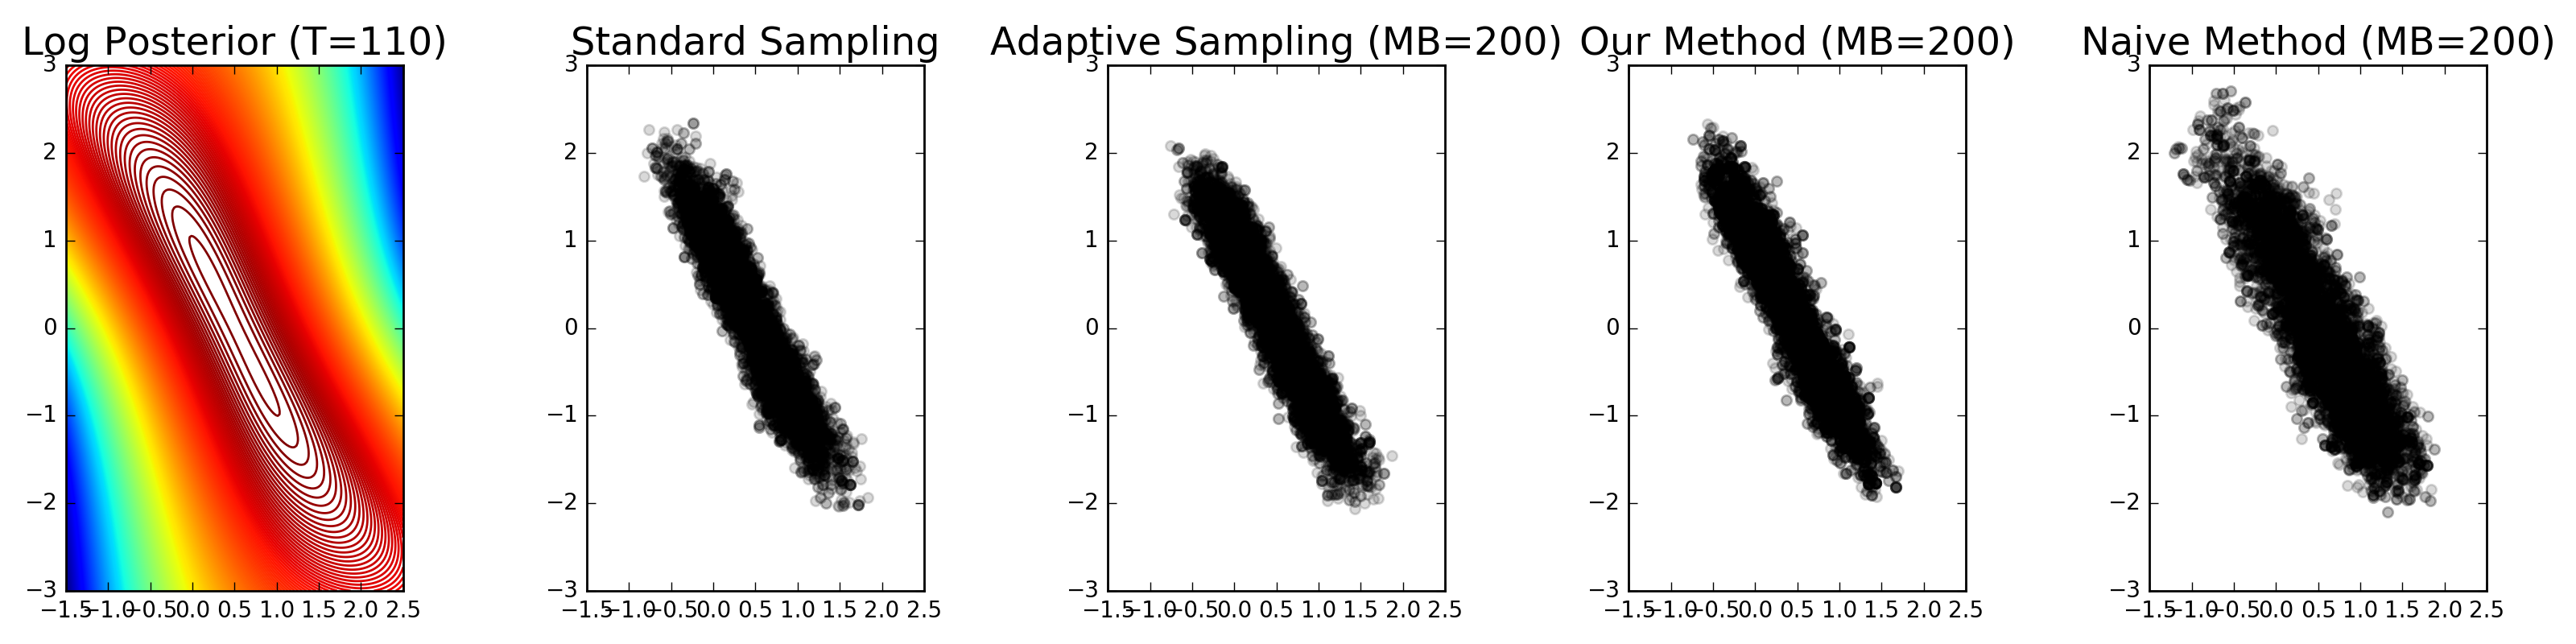
\includegraphics[width=1\linewidth]{cloud_v01.png}
    \caption{
    The log posterior contours (temperature 110) and three scatter plots of sampled $\theta$ values.
    }
    \label{fig:gauss_mix_1}
    %\vspace{-10pt}
\end{figure}

\begin{figure}[t]
    \centering
    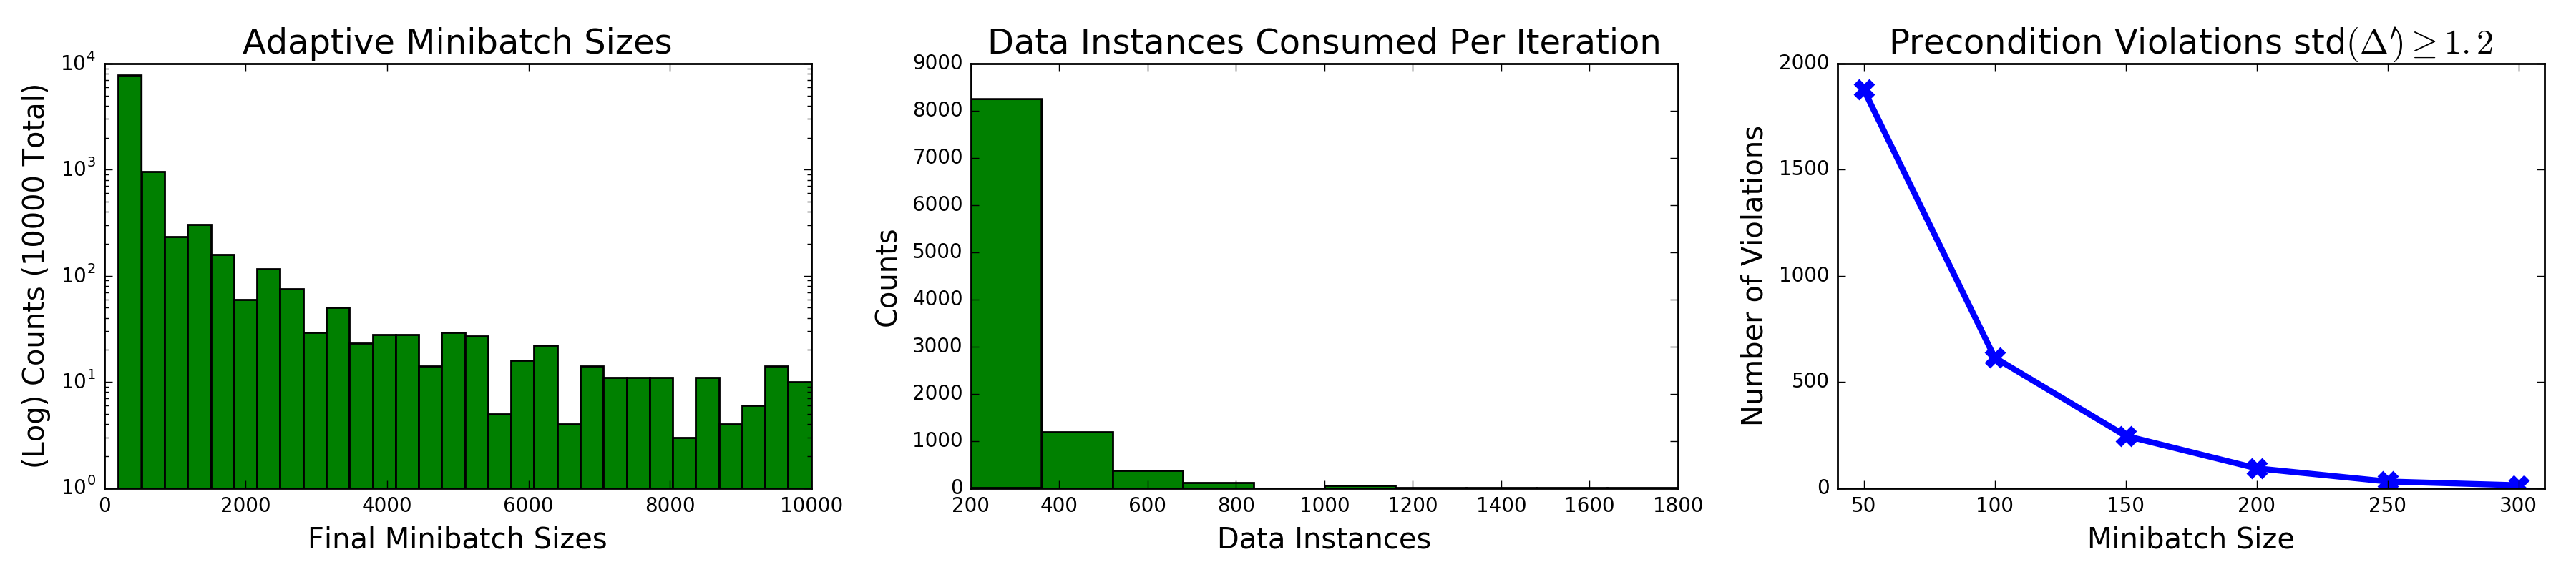
\includegraphics[width=1\linewidth]{adaptive_and_ours_information_v01.png}
    \caption{
    Histograms of minibatch sizes and ${\rm std}(\Delta')$ values, along with ``${\rm std}(\Delta')$
    violations'' (right).
    }
    \label{fig:gauss_mix_2}
    %\vspace{-10pt}
\end{figure}

Figure~\ref{fig:gauss_mix_1} shows three scatter plots of the resulting $\theta$ samples for the
three methods, with darker regions indicating a greater density of points. All three methods obtain
the same rough form of the posterior, so our MH test can indeed obtain the posterior just as the
other methods do.

Figure~\ref{fig:gauss_mix_2} (to the left) shows a histogram of the final minibatch sizes used by
the adaptive subsampling method each iteration (capped at 600 for readability).  Usually, the method
can make a decision with 200 samples. Occasionally, however, it must use all 10000 points, resulting
in more computation (some of it wasted). For this particular experiment, that happened eight times.  In
contrast, our method keeps the minibatch size fixed at 200, but requires that ${\rm std}(\Delta') <
1.2$. Figure~\ref{fig:gauss_mix_2} (in the middle) shows a histogram of the estimated ${\rm
std}(\Delta')$ values each iteration. Only 75 iterations resulted in ${\rm std}(\Delta') \ge 1.2$
and for those, we skipped the rest of the iteration (setting $\theta_{t+1}=\theta_t$). To smooth the
${\rm std}(\Delta')$ values, we use moving average updates. The third plot in
Figure~\ref{fig:gauss_mix_2} investigates the number of times ${\rm std}(\Delta') \ge 1.2$. For six
minibatch sizes (50, 100, 150, 200, 250, and 300), we ran MCMC with our MH test five times and
averaged the number of violations. As minibatch sizes increases, the number of violations decreases,
showing that our test is more applicable.


\subsection{Logistic Regression}\label{ssec:logistic}

We next use logistic regression for the binary classification of 1s versus 7s in the MNIST
dataset~\cite{lecun-mnisthandwrittendigit-2010}. The data has 12007 and 1000 training and testing
points, respectively (we used a random subset of the test data). The propose is again a random walk
with covariance matrix $0.1I$ for the $784\times 784$ identity matrix $I$. We initialize the
posterior temperature at $T_0=3000$, and decrease it according to $T_i = T_0 /\sqrt{i + 1}$ for
iteration $i \ge 1$. We set the minibatch size $m=50$ and compare our minibatch MH test with the
adaptive minibatch.

Figure~\ref{fig:logistic_fig} shows the prediction accuracy and log likelihood on the test set as a
function of the cumulative training data points processed. Our test increments the cumulative data
by a fixed amount per iteration, but the adaptive method may require more data per iteration.  We
see that our minibatch MH test is more efficient; it has similar or better performance while
consuming fewer data points.

\begin{figure}[t]
    \centering
    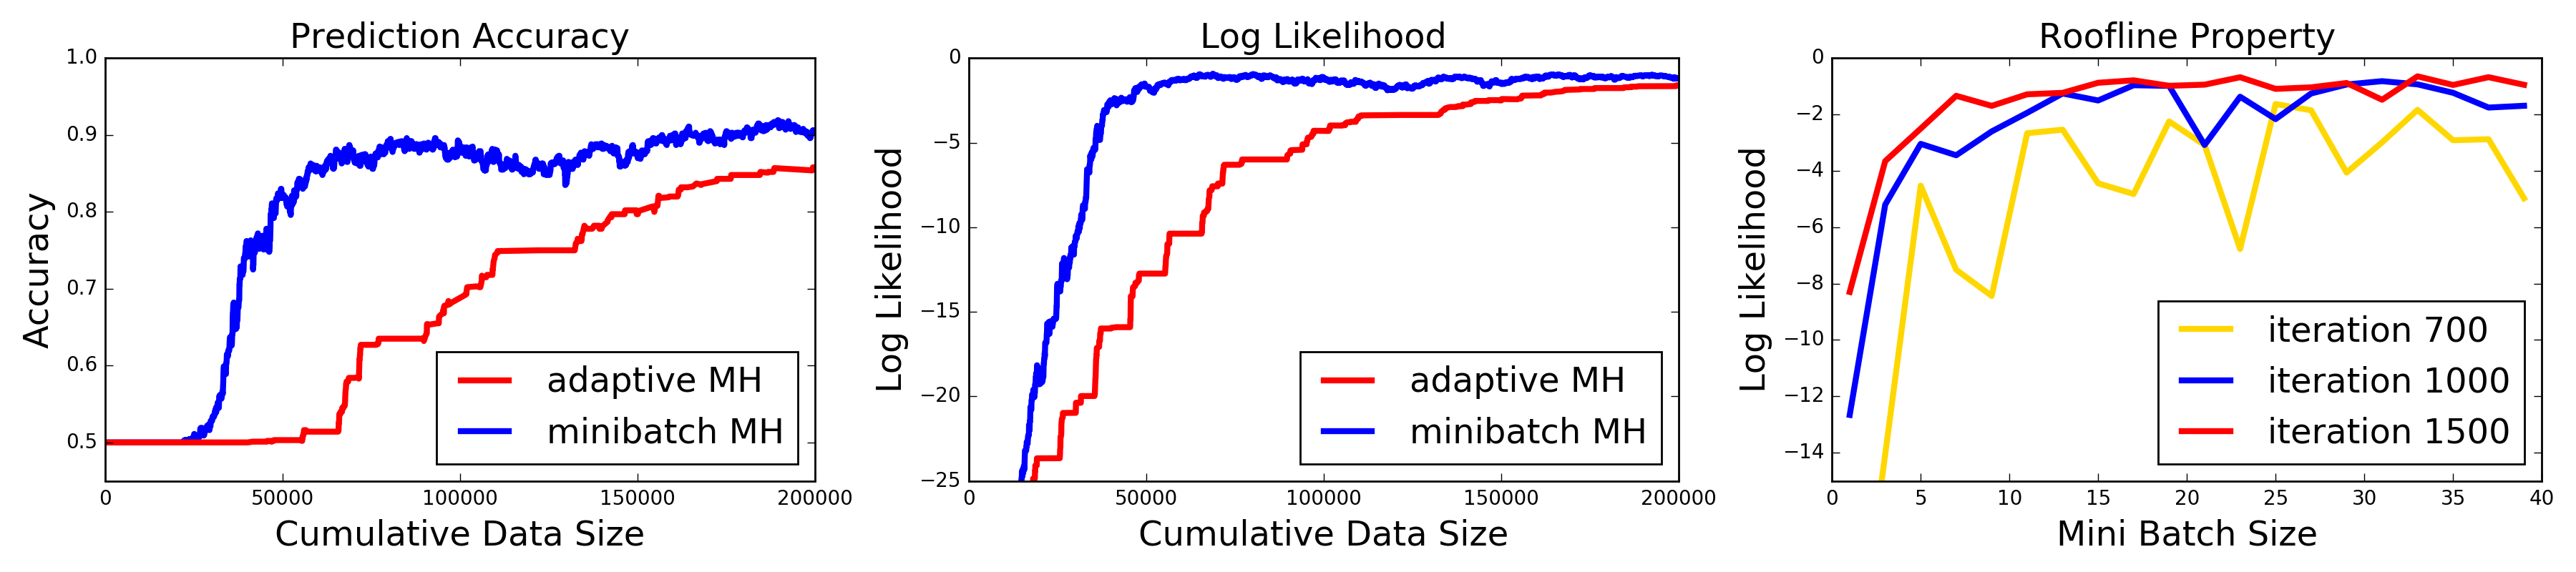
\includegraphics[width=1\linewidth]{exp2.png}
    \caption{Logistic regression performance (accuracy/log likelihood) and minibatch size analysis.}
    \label{fig:logistic_fig}
    %\vspace{-10pt}
\end{figure}

The third plot of Figure~\ref{fig:logistic_fig} shows performance based on minibatch size, when the
performance is evaluated on the test set after training iterations 700, 1000, and 1500. For all
three iteration counts, when the minibatch size increases beyond about 10, the performance of the
sampled data will not improve with a large minibatch size. This makes sense because the error of our
MH test is proportional to our estimation error of ${\rm std}(\Delta')$, and as the minibatch
increases, ${\rm std}(\Delta')$ decreases. Beyond a certain standard deviation threshold, the error
in our minibatch MH test is negligible.



\subsection{Neural Network Optimization}\label{ssec:nets}

In this experiment, we apply our minibatch MH test with a Stochastic Gradient Hamiltonian
Monte Carlo (SGHMC)~\cite{sghmc_2014} proposer to sample the parameter instances from a fully connected
neural network. We use the Higgs data set from the UCI dataset~\cite{Lichman:2013}. The network we
use for this binary classification problem has four layers and is fully connected. The first layer
is the input, the last layer is the softmax, and the intermediate layers apply the sigmoid
activation unit.  We also employ dropout and batch normalization~\cite{icml2015_ioffe15}.

For our comparison baseline, we train the same network architecture using the Adaptive Gradient
Descent method~\cite{adapGrad}. Since the frequencies of the features are quite different, we use
the same strategy in the Adaptive Gradient to rescale the gradient before apply SGHMC. We implement
our MH test and Adaptive Gradient in the open-source BIDMach project~\cite{canny2013bidmach}.  

Figure~\ref{fig:nnet_fig} illustrates our experiment results and reveals that SGHMC with our
minibatch MH test achieves higher log likelihood than the baseline. By comparing SGHMC with and
without our minibatch MH test, we see that our MH test has limited benefit. Because we decrease the
step size quickly, the acceptance rate of SGHMC is already high, so there is little need to test.
% Daniel's note: Haoyu said he cannot increase the step size without it violating the variance
% condition.

\begin{figure}[t]
    \centering
    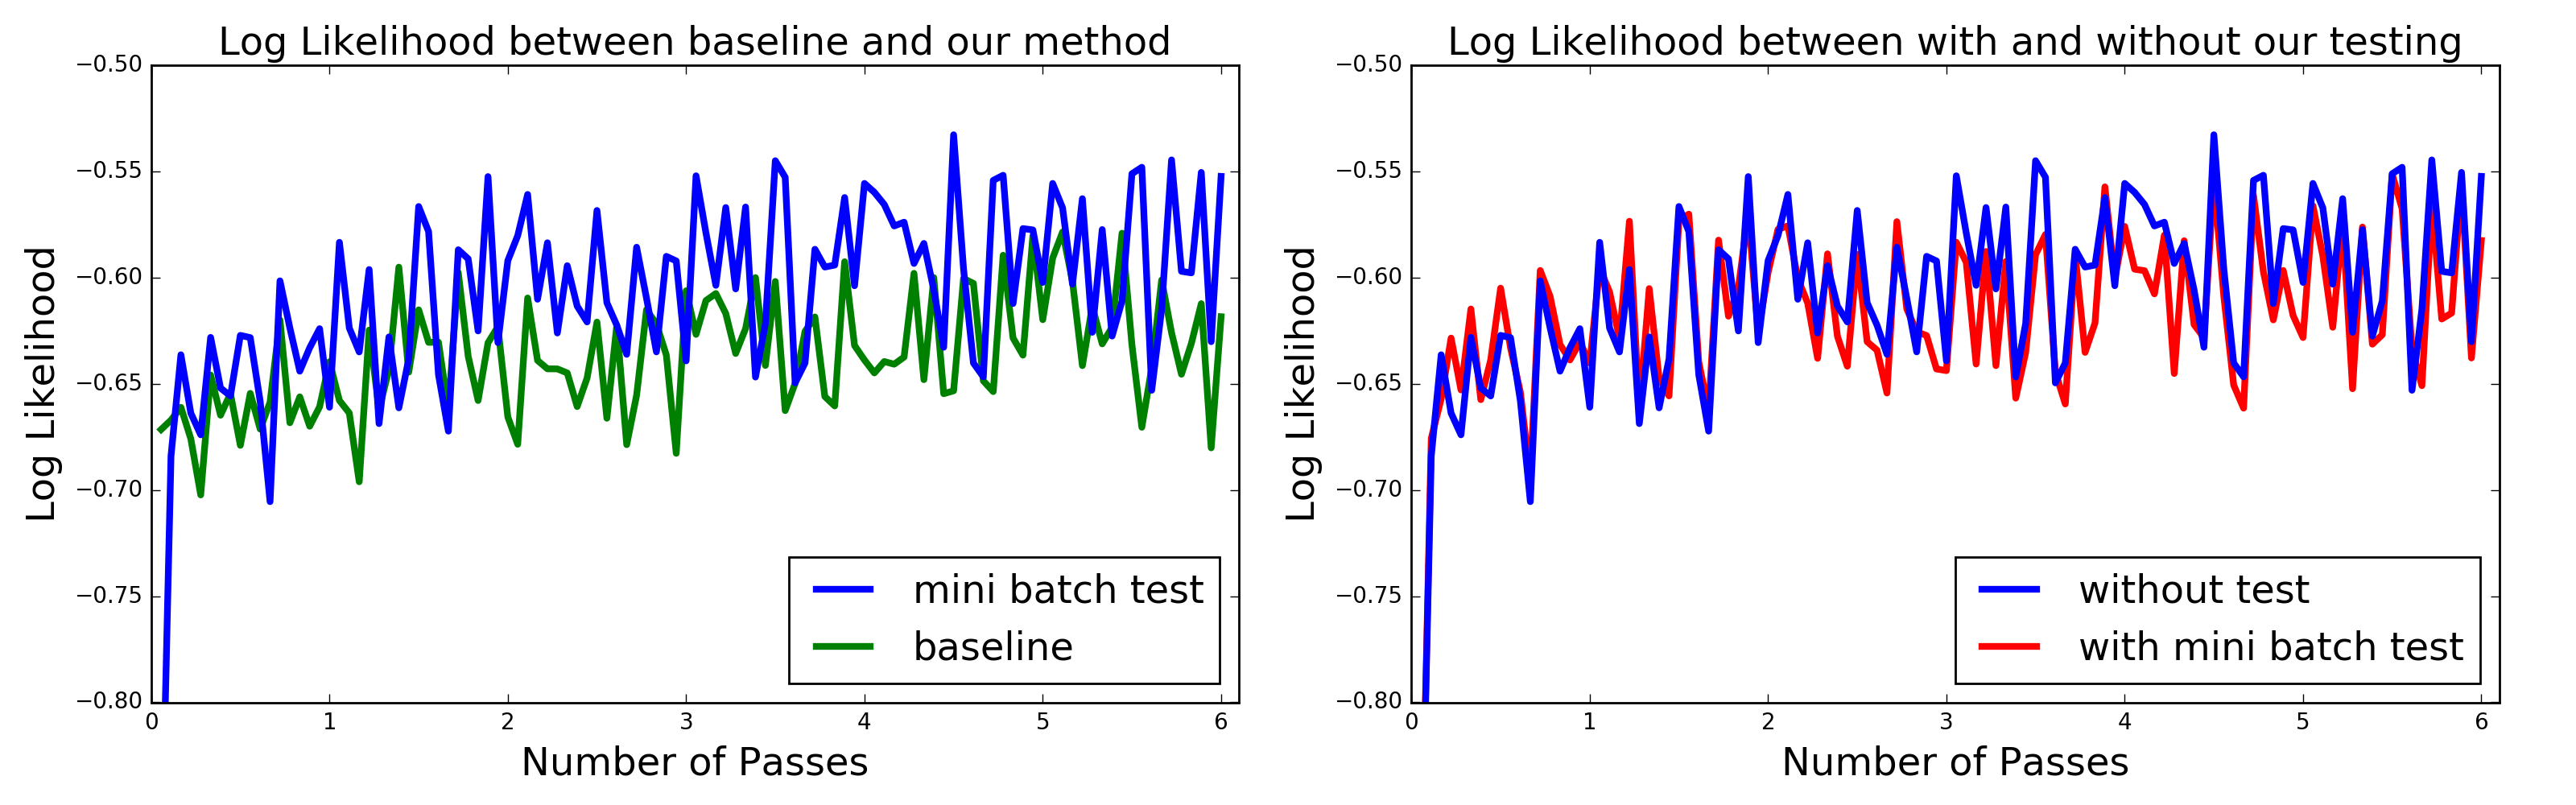
\includegraphics[width=1\linewidth]{exp3}
    \caption{Log likelihood versus number of passes for optimization of neural network.}
    \label{fig:nnet_fig}
    \vspace{-10pt}
\end{figure}




\section{Conclusions}\label{sec:conclusion}

In this paper, we have derived a new MH test for minibatch MCMC methods. We demonstrated how a
simple deconvolution process allows us to use a minibatch approximation to the full data tests. We
experimentally show the benefits of our test on Gaussian mixtures, logistic regression, and deep
learning.  Straightforward directions for future work include running more experiments with a
particular focus on investigation of the variance precondition.  More elaborate extensions include
combining our results with Hamiltonian Monte Carlo methods, providing a recipe for how to use our
algorithm (following the framework of~\cite{sgmcmc_2015}), or integrating parallel
MCMC~\cite{conf/uai/AngelinoKWSA14,conf/icml/AhnSW14} concepts.


\small
\bibliography{nips_2016}
\bibliographystyle{ieeetr}
\normalsize

\clearpage
\appendix

\begin{center}
{\Large Outline of Appendix}
\end{center}

In this appendix, we describe the following topics, with an emphasis on clarity and understanding:

\begin{itemize}[noitemsep]
    \item Some proof details on results in Section~\ref{sec:theory}.
    \item Detailed discussion of the experiment from Section~\ref{ssec:gaussians}.
    \item Detailed discussion of the experiment from Section~\ref{ssec:logistic}.
    \item Detailed discussion of the experiment from Section~\ref{ssec:nets}.
\end{itemize}

\section{Proofs}\label{app:proofs}

\subsection{Proof of Lemma~\ref{lem:theory1}}\label{app:theory1}

We first prove that the difference in our acceptance rates is bounded: $|P_a - P_a'| \leq 2\zeta
\ell$ for some small constant $\zeta > 0$. Given $X_\xi = \xi$ the distance $|P_a - P_a'|$ is:
\begin{align*}
|P_a - P_a'| &= |\Pr(\Delta + X >0) - \Pr(\Delta' + X_{\rm corr} > 0)|\\
& = | \Pr (\Delta + X > 0) - \Pr (\Delta + X_{\rm norm} + \xi + X_{\rm corr} >0) |    \\
&= |\Pr (\Delta + X > 0) -\Pr(\Delta + X + \xi >0)| = |F_X(-\Delta)- F_X(-\Delta - \xi)| \\
&= |\nabla F(-\Delta) \xi + o(\xi^2)| \leq  |\nabla F(-\Delta) \xi| +| o(\xi^2)| \leq 2|\nabla F(-\Delta)| |\xi| \leq 2\ell \xi,
\end{align*}
where the last line uses Taylor's Theorem ($o(\xi^2)$ represents higher-order terms that have
smaller absolute value) and the Triangle Inequality.  Since $|X_\xi| < \zeta$, $|P_a - P_a'| <
2 \zeta \ell$.

Next, we show the transition kernels at each step are bounded if we use the same proposer, i.e.
$\|P_i - P'_i\| \leq 2\zeta \ell$. We write $P_i(\theta_t \mid \theta') = P_a(\theta_t, \theta')
q(\theta'\mid \theta_t) + (1-P_a(\theta_t,\theta')) \delta_D(\theta' - \theta_t)$, where $\delta_D$
is the Dirac delta function. The total variation distance between two proposal kernels is
\begin{align*}
\|P_i - P'_i \| &= \int_{\theta'} \left| \int_{\theta_t}((P_a-P_a') q(\theta'|\theta_t) + (1-P_a - 1+P_a') \delta_D(\theta_t -\theta')) d\theta_t  \right| d\theta' \\
& = \int_{\theta'} \left| \int_{\theta_t} (P_a- P_a')(q(\theta'|\theta_t) - \delta_D(\theta_t - \theta')) d\theta_t \right|  d\theta'\\ 
& \leq 2 \zeta \ell \int_{\theta'} \left| \int_{\theta_t}(q(\theta'|\theta_t) + q(\theta_t|\theta')) d\theta_t \right| d\theta'= 2 \zeta \ell,
\end{align*}
as desired.

\subsection{Proof of Lemma~\ref{lem:theory2}}\label{app:theory2}

From Lemma~\ref{lem:gaussian}, only the $\sum_{i=1}^n (\log p(x_i\mid \theta') - \log p(x_i\mid
\theta_t))$ term brings randomness into $\Delta'$. To simplify the subsequent notation, we define
$g_i(\theta) = \log p(x_i\mid \theta)$, and $q_i = g_i(\theta') - g_i(\theta_t)$. Then by Taylor's Theorem:
\[
|q| = |g(\theta') - g(\theta_t)| = |\nabla g(\theta_t)^T(\theta' - \theta_t) + o(\theta' - \theta_t)^2| \leq 2\epsilon k.
\]
Thus, given $\theta$ and $\theta'$, the variance of $\Delta'$ can be written as:
\begin{align*}
{\rm Var}(\Delta') &= {\rm Var}\left[\sum_{i=1}^m g_i(\theta') - g_i(\theta_t)\right] = {\rm Var}\left(\sum_i^m q_i\right) \\
&= m {\rm Var} (q_i) + m(m-1) {\rm Cov}_{i \neq j}(q_i,q_j) \\
&= m{\rm Var}(q_i) - \frac{m(m-1)}{N-1} {\rm Var}(q_i) \\
&\leq 4\left(m - \frac{m(m-1)}{N-1}\right)k^2 \epsilon^2,
\end{align*}
as desired.

\subsection{Proof of Theorem~\ref{thm:theory3}}\label{app:theory3}

First, by Theorem 1 in~\cite{cutting_mh_2014}, $\|P_i \circ D_0 - \pi\| \leq \eta \|D_0
- \pi\|$ and $\|P_i-P'_i\| \leq \epsilon_i C$, the norm between the stationary distribution is $\|\pi
- \pi_i'\|\leq \frac{\epsilon_i C}{1-\eta}$.

Second, by Theorem 3.6 in~\cite{yang2013sequential}, we have  $\| P_t' \circ P_{t-1}' \circ \cdots
\circ P_1' D_0 - \pi_t \| \leq \sum_{s=1}^t \{\prod _{u=s+1}^t \rho_u (1-\alpha_u)\} \rho_s
\alpha_s$, where $\alpha = \frac{\epsilon_i C}{1-\eta}$. Thus, we get:
\begin{align*}
 \| P_t' \circ \cdots \circ P_1' D_0 - \pi_0 \| &\leq \|P_t' \circ \cdots \circ P_1' D_0 - \pi_t\| + \|\pi_t - \pi_0\| \\
 &\leq \sum_{s=1}^t \left\{\prod _{u=s+1}^t \rho_u (1-\alpha_u)\right\} \rho_s \alpha_s + \alpha_t,
\end{align*}
as desired.




\section{Gaussian Mixture Experiment Details}\label{app:gaussian}

\subsection{Mathematical Assumptions}

We borrow this example from~\cite{langevin_2011}. Our parameter is a 2-D vector $\theta =
(\theta_1, \theta_2)$, where
\begin{equation}
\theta_1 \sim \mathcal{N}(0, \sigma_1^2) \quad \mbox{ and } \quad \theta_2 \sim \mathcal{N}(0, \sigma_2^2)
\end{equation}
where $\mathcal{N}$ indicates the normal distribution (more generally, the multivariate normal). We
consider the above as our prior. Following~\cite{langevin_2011}, we set $\sigma_1^2 = 10$ and
$\sigma_2^2=1$, so the covariance matrix of $\theta$ is $\Sigma = {\rm diag}(10,1)$. Therefore, the
log prior probability we endow on $\theta$ is
\begin{equation}
\log p(\theta) = \log \left(\frac{1}{2\pi\sqrt{10}}\right) - \frac{1}{2}\theta^T\Sigma^{-1}\theta.
\end{equation}
To generate the data, we use the following Gaussian mixture with tied means:
\begin{equation}\label{eq:x_points}
x_i \sim \frac{1}{2}\mathcal{N}(\theta_1, \sigma_x^2) + \frac{1}{2}\mathcal{N}(\theta_1+\theta_2, \sigma_x^2)
\end{equation}
where, again following~\cite{langevin_2011}, we set $\sigma_x^2 = 2$. This means the log likelihood
of a single data instance is
\begin{equation}
\log p(x_i \mid \theta) = \log\left(\frac{1}{4\sqrt{\pi}}\right) +
\log\left(\exp\left(-\frac{1}{4}(x_i - \theta_1)^2\right) + \exp\left(-\frac{1}{4}(x_i -
(\theta_1+\theta_2))^2\right)\right)
\end{equation}
Here is the problem statement. Given some number of i.i.d. data points $x_1, x_2, \ldots, x_N$
generated according to~(\ref{eq:x_points}), determine the posterior distribution\footnote{Note that,
as is typical with Bayesian analysis, we do not concern ourselves with the denominator of the
original (non-log) posterior.} of $\theta$:
\begin{equation}\label{eq:log_post}
\log p(\theta \mid x_1,\ldots,x_N) = \log p(\theta) + \sum_{i=1}^N\log p(x_i \mid \theta).
\end{equation}
Alternatively, if there are too many data points, we may opt to instead pick a point estimate of
$\theta$, generally the MAP estimate. (If $N$ is extremely large, it will cause the posterior to
peak sharply at its modes, reducing distribution estimates to point estimates.) Note that in many
cases, we will need to take a \emph{minibatch estimate} of~(\ref{eq:log_post}). In that case, the
literature generally uses
\begin{equation}\label{eq:scaling_factor}
\log p(\theta \mid x_1,\ldots,x_N) \approx \log p(\theta) + \frac{N}{n} \sum_{i=1}^n\log p(x_i \mid \theta).
\end{equation}
where we only use $n \ll N$ samples, but we must scale up the likelihood contribution by $N/n$. If we
didn't add this scaling factor, then the contribution of the likelihood terms would be weaker. There
is another thing we need to consider about that, which is the \emph{temperature} of our
distribution. In general, we will want to add $T > 1$ so that our posterior is
$p(\theta)((\prod_{i=1}^n p(x_i\mid \theta))^{N/n})^{1/T}$, resulting in the log
posterior of 
\begin{equation}\label{eq:log_prior_temp}
\log p(\theta \mid x_1,\ldots,x_N) \approx \log p(\theta) + \frac{1}{T}\frac{N}{n} \sum_{i=1}^n\log p(x_i \mid \theta).
\end{equation}
which has the extra $1/T$ to decrease the scale factor.  Equation~(\ref{eq:log_prior_temp}) is what
we will be using for our experiments, because we need to consider warmer distributions.
{\color{blue} Daniel: not totally confident on this but I'll try.}

Finally, recall earlier that we needed to define $\Delta$. In our context, $\Delta$ is:
\begin{align}
\Delta &= \log \left(\frac{f(\theta') q(\theta_t \mid \theta')}{f(\theta_t) q(\theta'\mid \theta_t)} \right) \\
&= \log p(\theta') - \log p(\theta_t) + \sum_{i=1}^N(\log p(x_i \mid \theta') - \log p(x_i \mid \theta_t)) + \log\left(\frac{q(\theta_t \mid \theta')}{q(\theta' \mid \theta_t)}\right).
\end{align}
But again, with \emph{minibatches} of data, we usually do not sum over all $N$ terms and instead sum
over $n$ terms, but with the extra $(1/T)(N/n)$ scaling factor, from
Equation~(\ref{eq:log_prior_temp}). We generally denote that approximation as $\Delta'$ in the paper.

\subsection{Experiment Observations}

\begin{figure}[t]
  \centering
  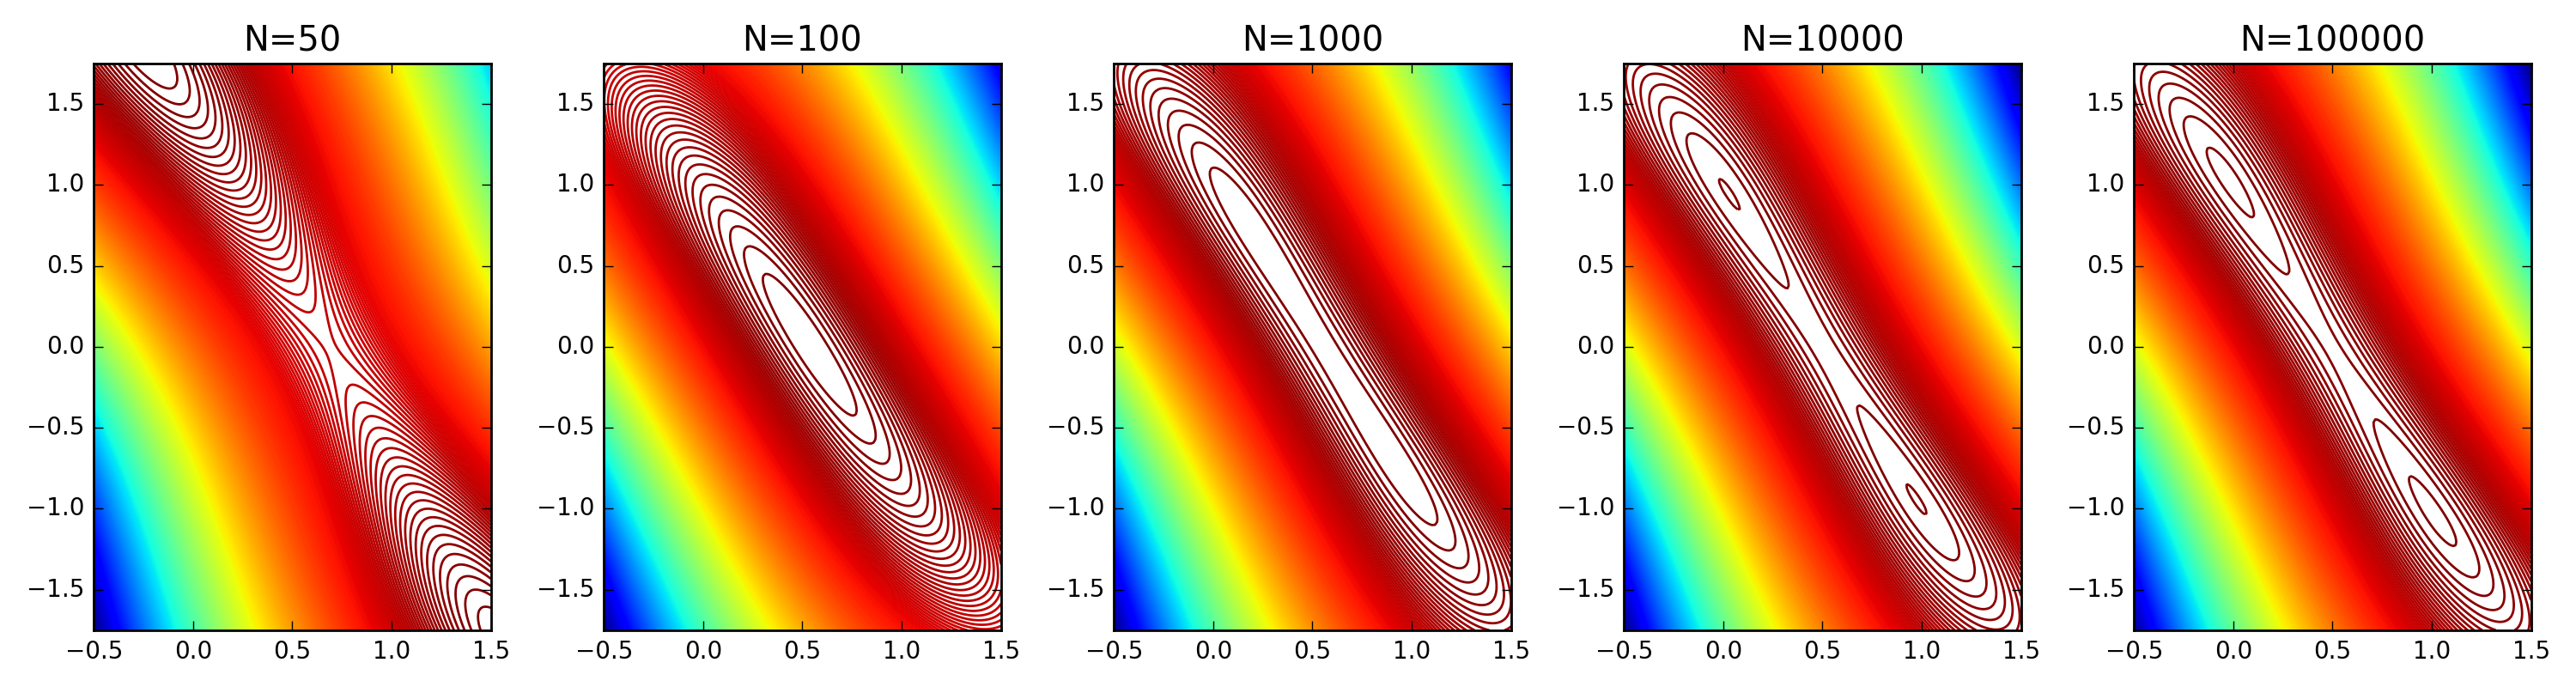
\includegraphics[width=1\linewidth]{contour_v1}
  \caption{The posterior distribution, from 50 to 100k samples, with temperature set at 1.}
  \label{fig:contour1}
\end{figure}
\begin{figure}[t]
  \centering
  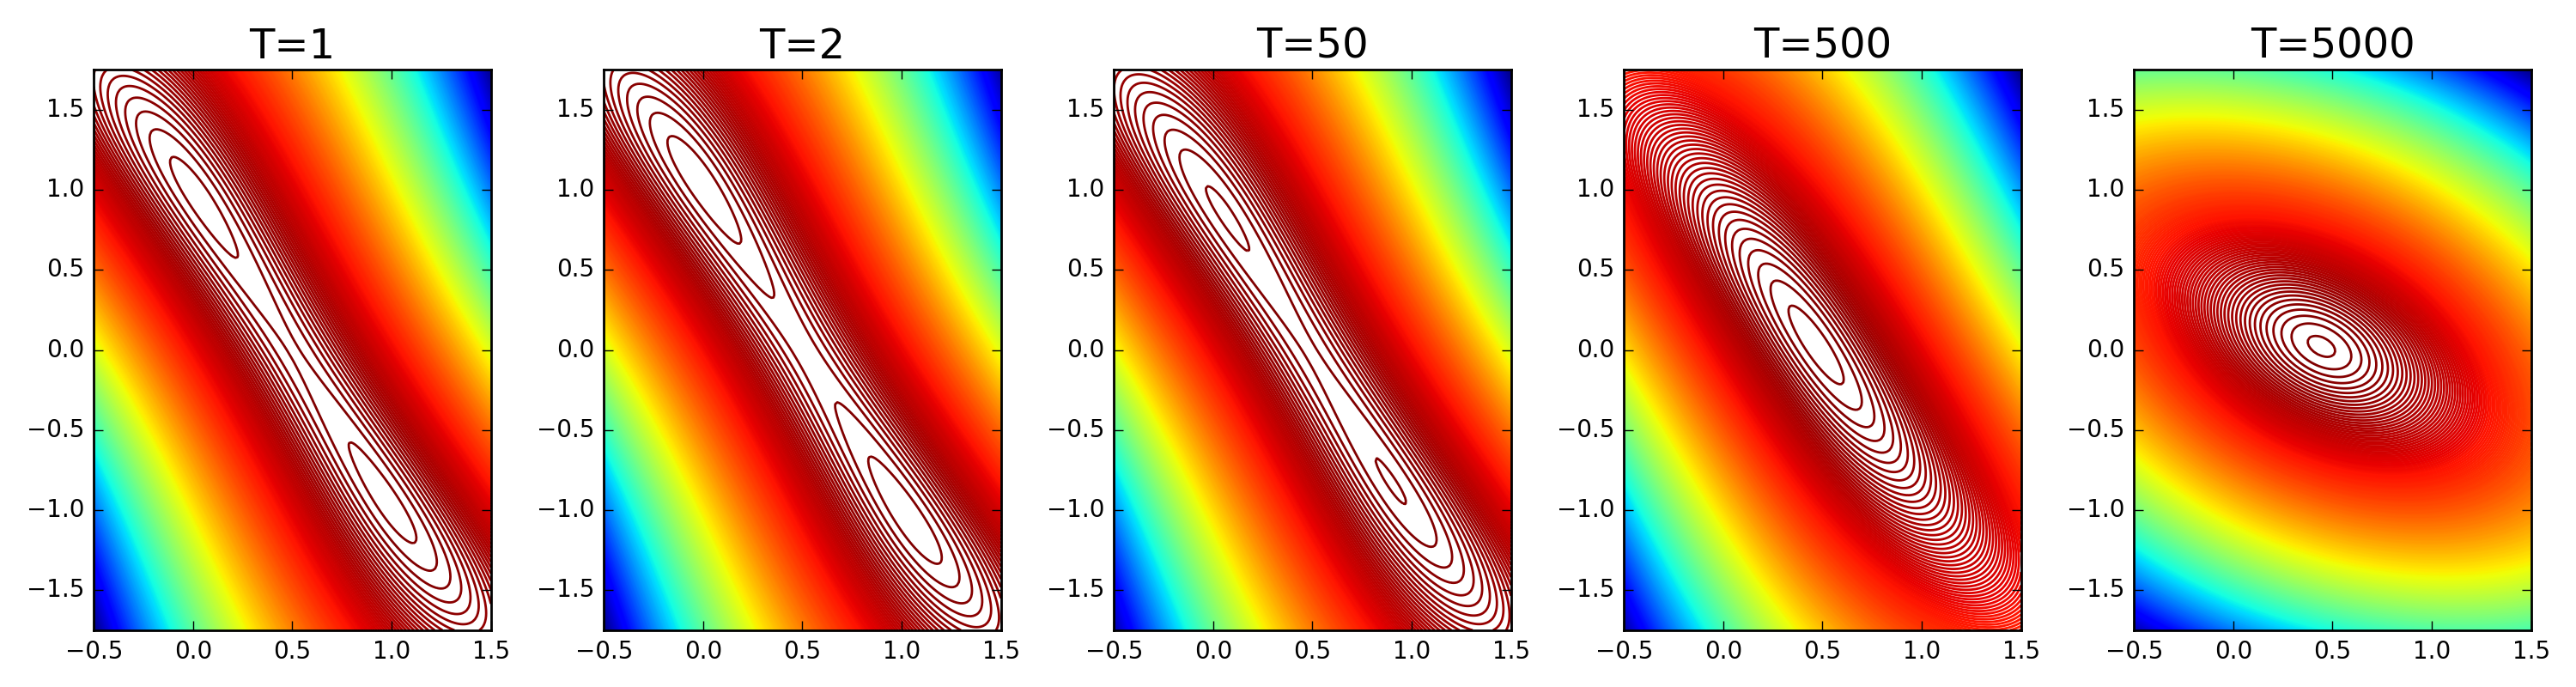
\includegraphics[width=1\linewidth]{contour_v2}
  \caption{The posterior distribution, with $N=10000$ but with temperature $T$ varying.}
  \label{fig:contour2}
\end{figure}

In this experiment, we compare our method with the one from~\cite{cutting_mh_2014}, hereafter called
the ``adaptive sampling approach''. We apply them to the Gaussian Mixture model previously
discussed.

Figure~\ref{fig:contour1} shows simulated contour plots of the posterior based on the $N$ data
points, for varying $N$, with the temperature set at $T=1$. Note that because we're using all $N$
points here, the scale factor $N/n=1$. As $N$ increases, the posterior converges to a multimodal
distribution with modes at $(0,1)$ and $(1,-1)$. 

Figure~\ref{fig:contour2} is similar, except this time we fix the number of samples at $N=10000$,
but show how changing the temperature $T$ affects the distribution. A larger $T$ implies a flatter
posterior, one that (weakly) peaks in between the two true modes.

Our ultimate goal is to either (a) get a posterior distribution that covers the posterior well, or
(b) to get samples that stay trapped at a mode, for a point estimate of $\theta$.  Whether our goal
is (a) or (b) depends on our objectives and the context of the problem (e.g., big data usually
implies (b) is OK even if it would not satisfy the average Bayesian).

For both our method and the adaptive sampling method, we use random walk proposals. (Thus, the term
in $\Delta$ containing the $q$s disappears.)  Random walk proposals are bad, but since the proposal
is poor, good performance can only be obtained with a strong MH test, hence why we can use this as a
reasonable starting benchmark.

We test use the following settings:

\begin{itemize}[noitemsep]
    \item We use $N=10000$ samples of $x_i$.
    \item The covariance of the Gaussian random walk is ${\rm diag}(0.1, 0.1)$.
    \item We use 10000 iterations. One iteration involves one $\theta'$ proposal and a test to
    accept/reject.
    \item The minibatch size is set at 100, so it is one percent of the total data. For the
    adaptive sampling approach, this is the amount that the minibatch size would keep increasing if
    we needed more precision. Our approach, of courses, keeps the size fixed.
    \item For adaptive sampling, the tolerance for deciding on a test is 0.05. The temperature for
    that is also set at $T=1$ because that algorithm was not designed to deal with temperatures.
    \item For our approach, to get an estimate of the standard deviation of $\Delta'$ (remember,
    $\Delta'$ is a minibatch approximation of $\Delta$) we take five other minibatches (randomly
    selected from the data) and take the standard deviation of those values.
\end{itemize}

For our approach, we run using three different temperature values, $T=1$, $T=10$, and $T=100$.

Figure~\ref{fig:scatter} compares scatter plots of the ``Cutting the MH'' test (hereafter called
``adaptive minibatch'') versus ``Our Method'', where we use three different temperature settings.
There doesn't seem to be too much noticeable difference in our method for the three different
temperature setting values, but our approach is a lot different from the adaptive sampling method
(this is because of rejection rates, more on that later).

\begin{figure}[ht]
  \centering
  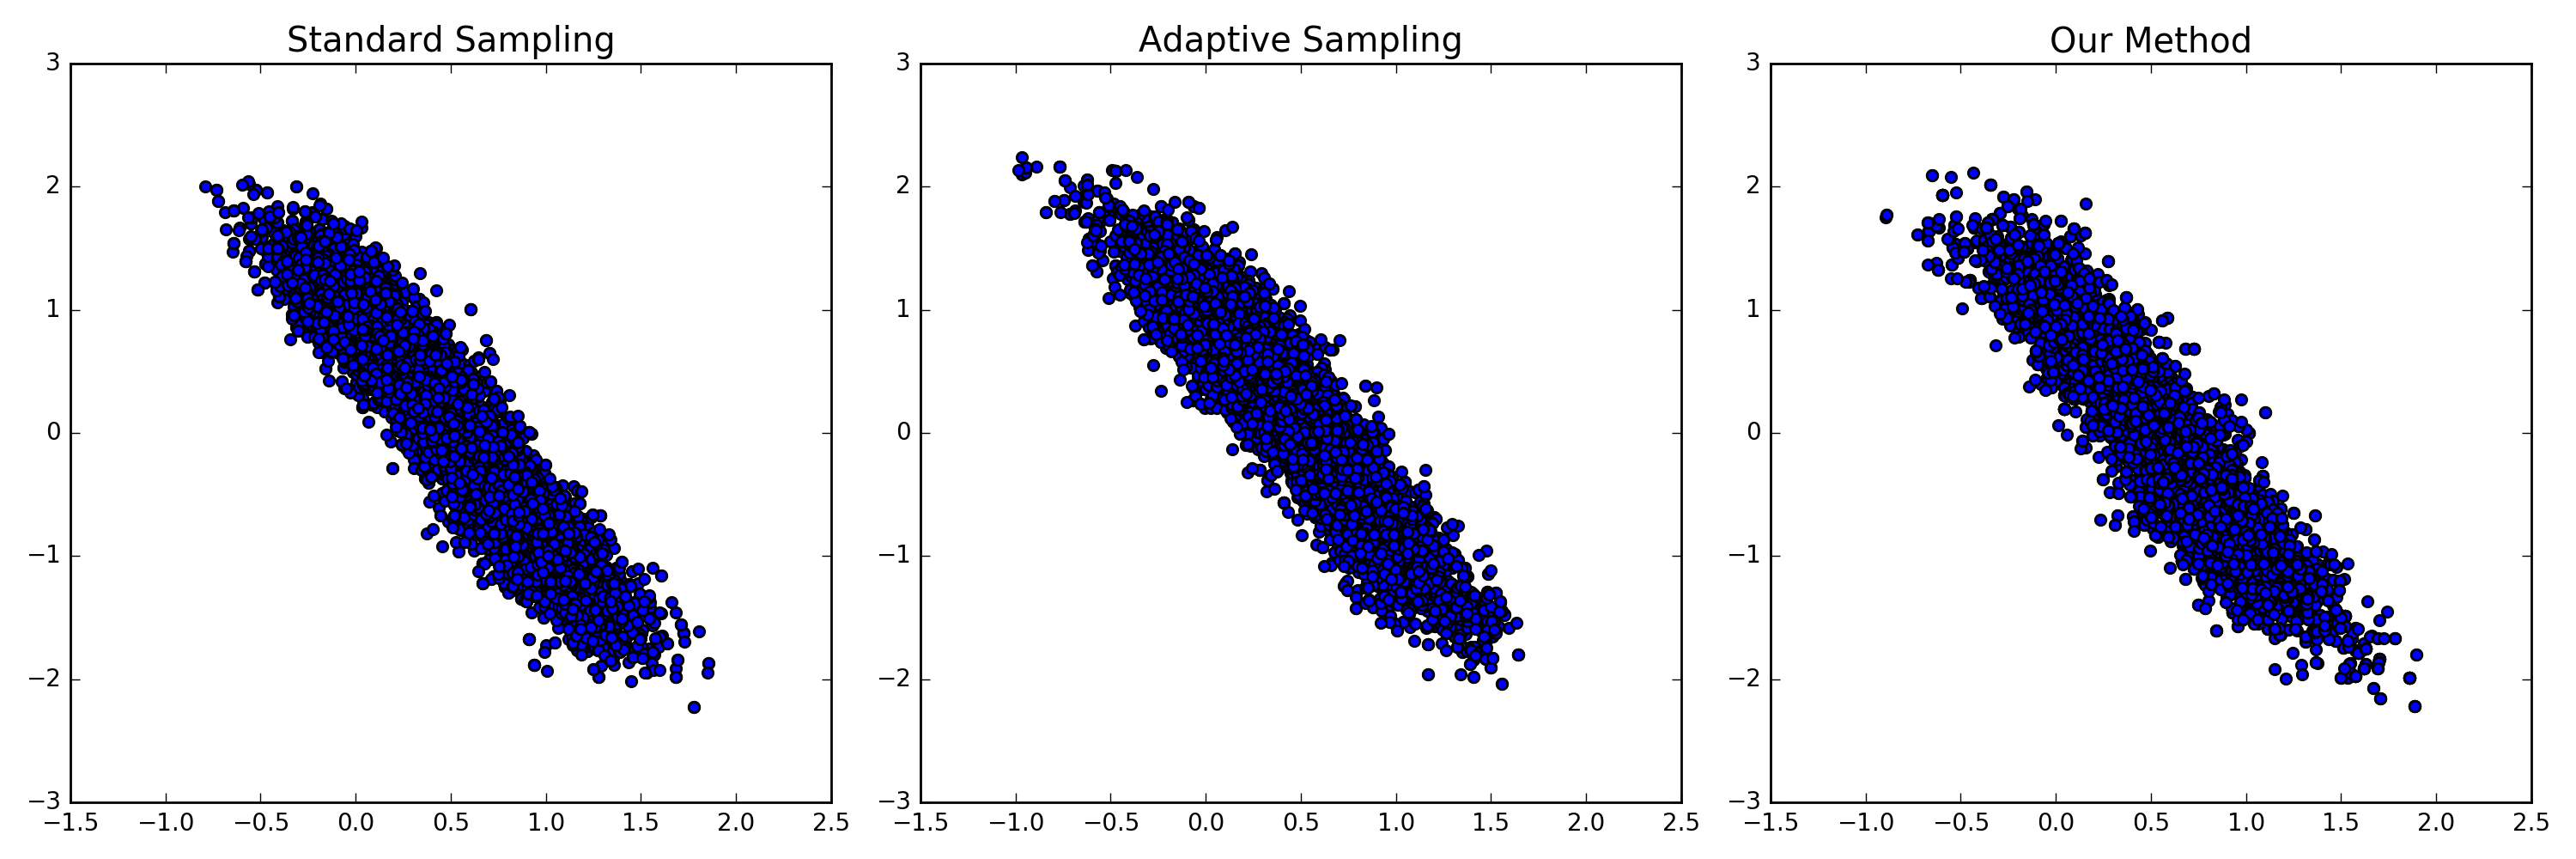
\includegraphics[width=1\linewidth]{scatter_v01}
  \caption{Scatter plots of accepted $\theta$ for (in order) the adaptive sampling approach, and our
  method (temperatures 1, 10, and 100).}
  \label{fig:scatter}
\end{figure}

Before taking a look at our approach, we first examine the adaptive sampling approach. \textbf{That
approach rejected a lot of samples; out of 10000 iterations, it only accepted 773 times}.
Figure~\ref{fig:mb_sizes} describes the histograms of the adaptive minibatch's batch sizes. (Note
that the histogram y-axis values are different.) In many cases, using the initial batch size of 100
sufficed to make an accept/reject decision, but sometimes, this method needed to use the entire 10k
data set. Decreasing the tolerance (from its current 0.05 value) would have required larger
minibatches. Incidentally, it makes sense that the method rejects a lot of samples, because the
random walk proposal usually provides us with poor points.

\begin{figure}[ht]
  \centering
  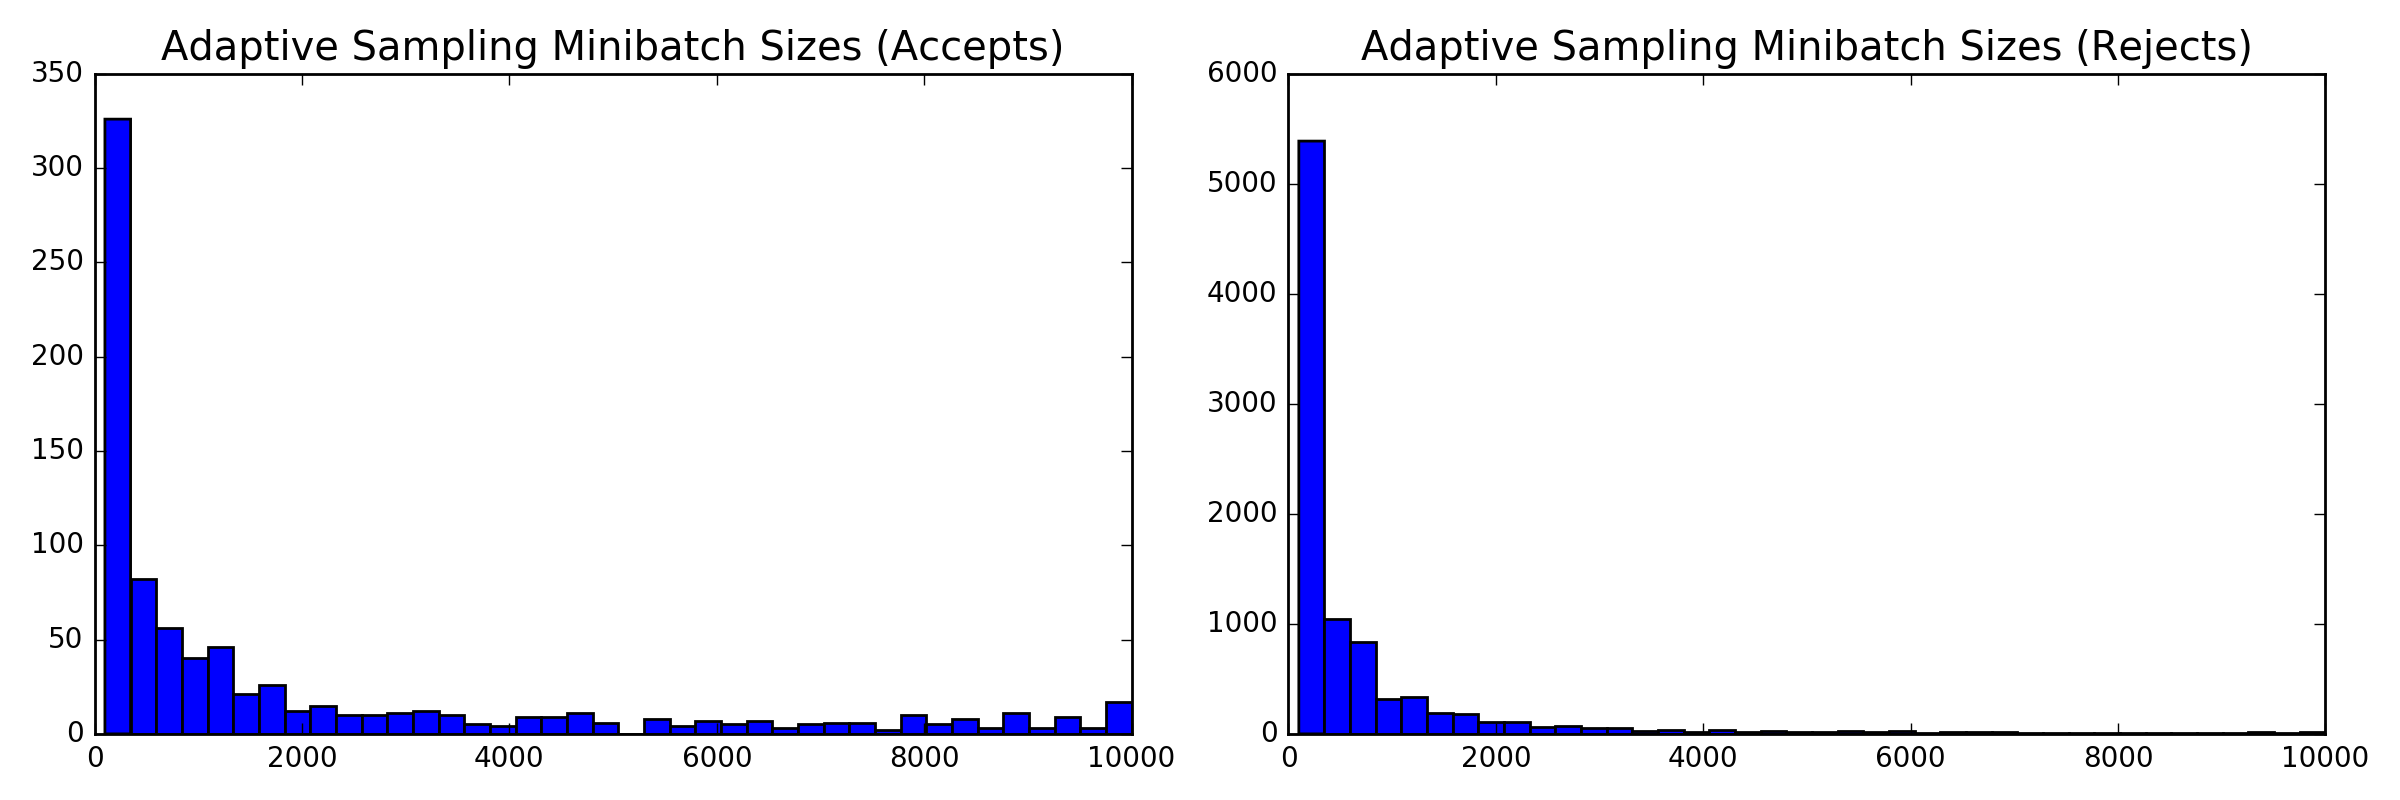
\includegraphics[width=0.75\linewidth]{adaptive_sampling_sizes_v01.png}
  \caption{Minibatch sizes for adaptive sampling when it was accepting or rejecting.}
  \label{fig:mb_sizes}
\end{figure}

Now we analyze our approach in more detail. Our method accepts far more samples than the adaptive
sampling method, \textbf{accepting 3285, 3318, and 3332 out of 10k}, for temperature values 1, 10,
and 100, respectively.

For diagnostics purposes, Figures~\ref{fig:diagnostics1},~\ref{fig:diagnostics2},
and~\ref{fig:diagnostics3} express histograms (for all three temperature runs) of the $\Delta'$,
${\rm std}(\Delta')$, and $X_{\rm corr}$ values, respectively.

There are a few immediate observations. First, increasing the temperature size by a factor of 10
will decrease $\Delta'$ by a factor of 10, which makes sense. That will also directly affect the
standard deviation estimate of $\Delta'$. Our $X_{\rm corr}$ distribution is symmetric about zero,
which is also expected (and it also exhibits a decrease in a factor of 10 for an increase
in temperature).

{\color{blue}
Daniel: One concern I have is that our $\Delta'$ values do not seem to be ``sufficiently negative''. If our
$\Delta'$ values are negative (but large in absolute value) that means our MH test will reject more
often. But then this raises another concern: didn't we say at one point that we \emph{should} be
getting high acceptance rates, around 50 percent (in part because of the shape of the logistic
function)? Doesn't that depend on the quality of the proposal distribution? If our method is
designed to accept a lot regardless of the proposal distribution, I don't see how its performance
can be considered equal to the adaptive sampling approach, or even a standard MH test. In fact, the
best observation I can derive from this is that our approach and the adaptive sampling (or any
standard MH test) will accept the high likelihood cases, but our case will accept the borderline
ones more often.
}

\begin{figure}[ht]
  \centering
  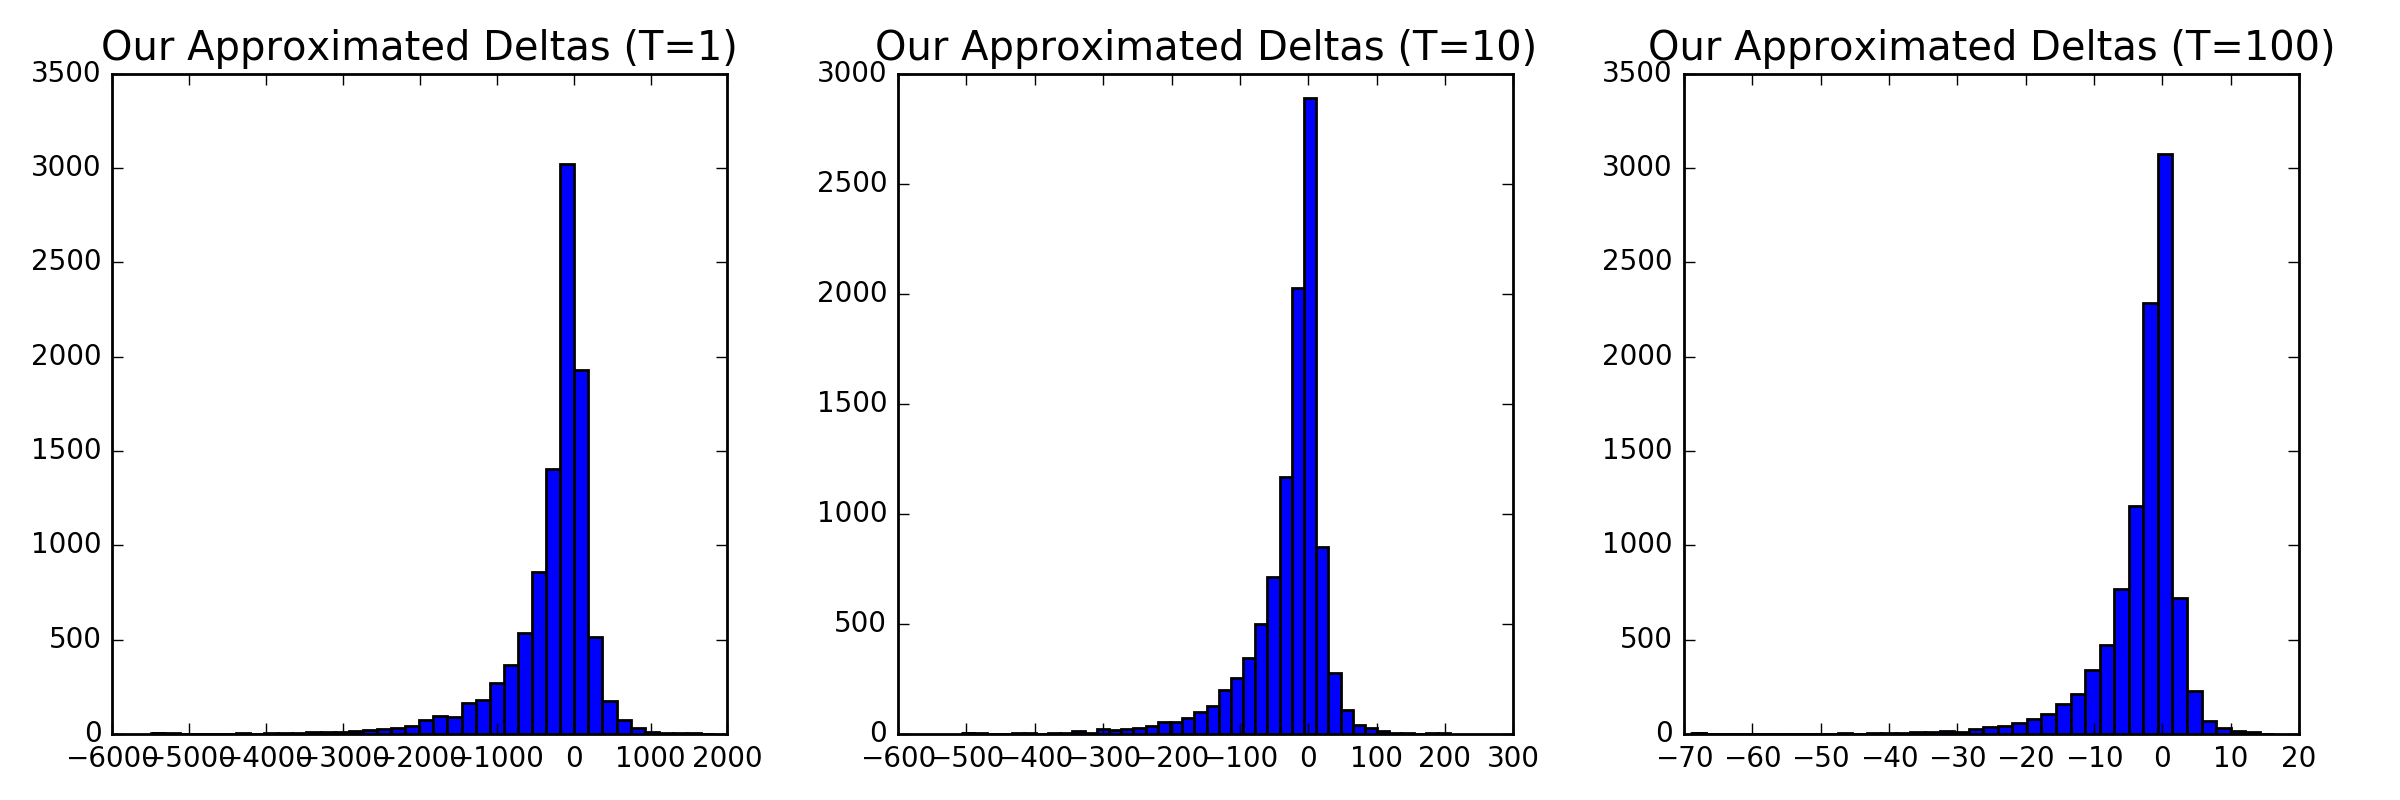
\includegraphics[width=1\linewidth]{our_deltas_v01.png}
  \caption{Our $\Delta'$ values for three different temperature values.}
  \label{fig:diagnostics1}
\end{figure}

\begin{figure}[ht]
  \centering
  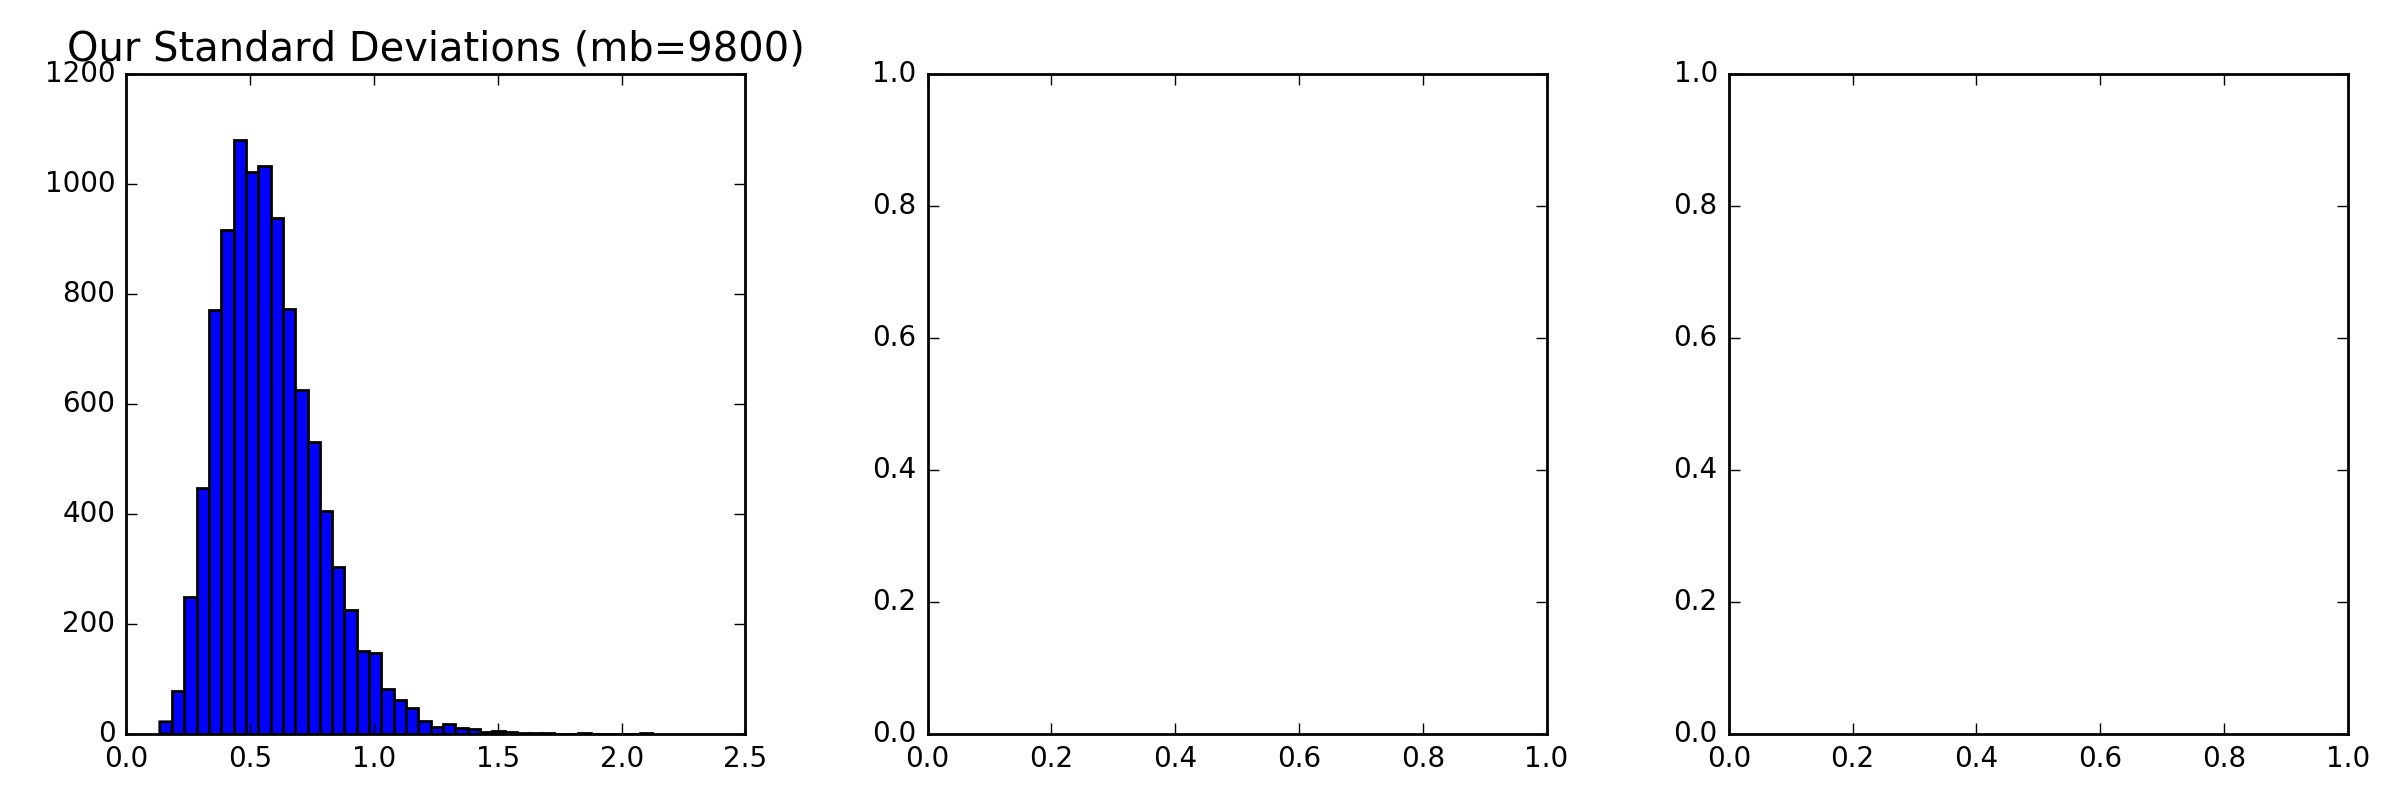
\includegraphics[width=1\linewidth]{our_sds_v01.png}
  \caption{Our ${\rm std}(\Delta')$ values for three different temperature values.}
  \label{fig:diagnostics2}
\end{figure}

\begin{figure}[ht]
  \centering
  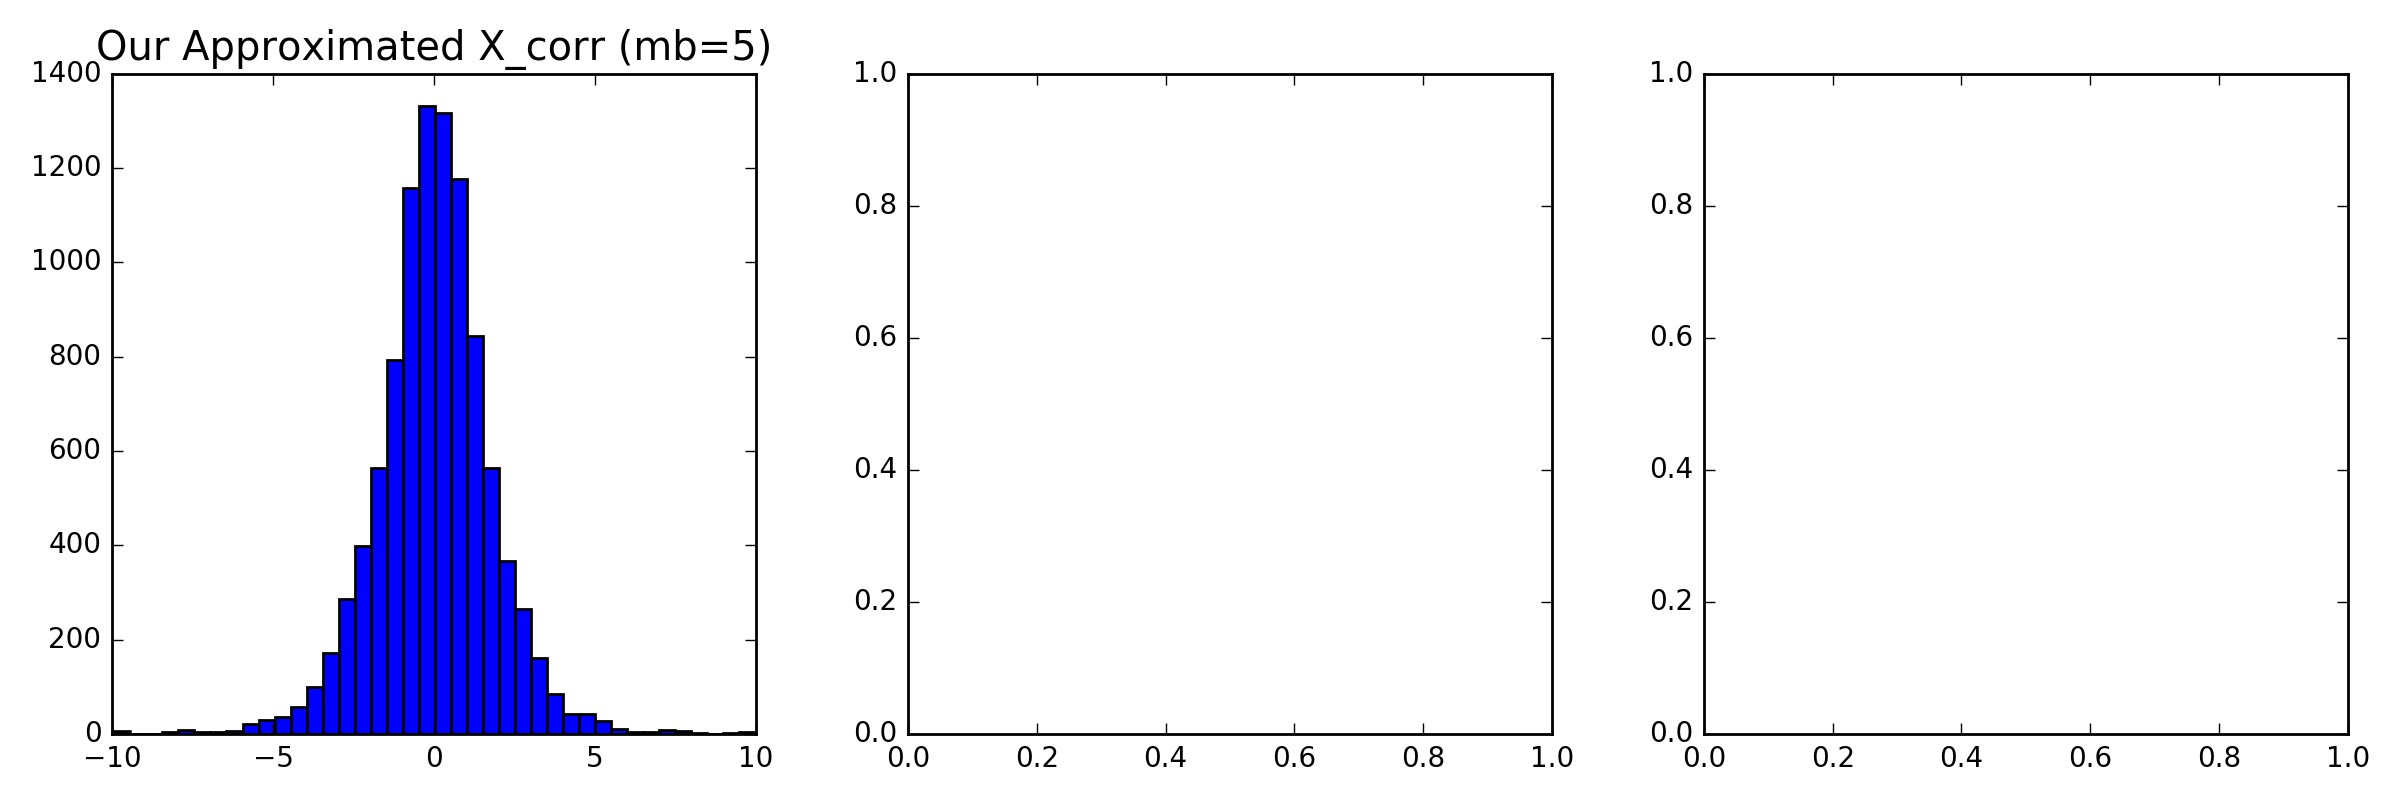
\includegraphics[width=1\linewidth]{our_xcorrs_v01.png}
  \caption{Our $X_{\rm corr}$ values for three different temperature values.}
  \label{fig:diagnostics3}
\end{figure}



\section{Logistic Regression Experiment Details}\label{app:logistic}

We applied our minibatch Metropolis Hastings algorithm to a Bayesian logistic regression model,
comparing with the adaptive sampling method. We tested both our method and the adaptive sampling
method using a random walk proposer $q(\theta \mid \theta_t) = N (\theta_t, \sigma^2)$. Since the
random walk proposer does not contain any information about the target distribution, it only relies
on the Metropolis-Hastings test to converge to the correct distribution. Therefore, random walk
proposer is the ideal choice for illustrating our algorithm and comparing with the adaptive sampling
method.

\section{Neural Network Experiment Details}\label{app:nnet}

{\color{blue}
Daniel: TODO
}

% Daniel: here are example LaTeX codes for figures and tables if we want to use them.
%\begin{figure}[h]
%  \centering
%  \fbox{\rule[-.5cm]{0cm}{4cm} \rule[-.5cm]{4cm}{0cm}}
%  \caption{Sample figure caption.}
%\end{figure}
%\begin{table}[t]
%  \caption{Sample table title}
%  \label{sample-table}
%  \centering
%  \begin{tabular}{lll}
%    \toprule
%    \multicolumn{2}{c}{Part}                   \\
%    \cmidrule{1-2}
%    Name     & Description     & Size ($\mu$m) \\
%    \midrule
%    Dendrite & Input terminal  & $\sim$100     \\
%    Axon     & Output terminal & $\sim$10      \\
%    Soma     & Cell body       & up to $10^6$  \\
%    \bottomrule
%  \end{tabular}
%\end{table}
%\usepackage[pdftex]{graphicx} ...
%\includegraphics[width=0.8\linewidth]{myfile.pdf}

\end{document}
